\documentclass{UoYCSproject}
\usepackage[dvipsnames]{xcolor}
\usepackage{mathptmx}
\usepackage{booktabs}
\usepackage{gensymb}
\usepackage{hyperref}
\usepackage{tikz}
\usepackage{wrapfig}
\usepackage{fancyvrb}
\usepackage{tikz}
\usepackage{filecontents}
\usepackage{pgfplots, pgfplotstable}
\usepackage{float}
\usepackage{listings}
\usepackage{graphicx}

% Text font
\usepackage{charter}

% \usepackage{newcent}
% \usepackage{fourier}
% \usepackage{mathpazo}% Palatino

\usepgfplotslibrary{statistics}

\usetikzlibrary{shapes.geometric}
\usetikzlibrary{calc}


\graphicspath{{images/}}

\newcommand{\pep}{p\texorpdfstring{$\equiv$}{E}p~}
\newcommand{\cisco}{cisco_images}
\newcommand{\ciscoImageScale}{0.7}

\addbibresource{references.bib}

\author{Aidan Fray}
\title{Investigating the Security of  \pep's Trustword PGP Fingerprint Encoding}
% \date{10 September 2019}
\supervisor{Siamak Fayyaz Shahandashti}
\CYB

% \dedication{To all students everywhere}

% \acknowledgements{
%   TODO
% }


\newcommand{\todo}[1]{
  \textit{\color{ForestGreen}\textbf{TODO: } #1}
}

% Used to display graphs for experiment one
\newcommand{\tally}[1]{%
\begin{tikzpicture}
  \begin{axis}[
    ymin=0,
    ymax=200,
    xtick={1,2,3,4,5},
    width=1\textwidth,
    grid,
    xlabel={Phonetic raiting},
    ylabel={Oucurrance}
  ]
    \addplot[ybar, fill=blue] table[ 
        col sep=comma,
        y=occurrence, 
        x=rating] 
    {#1};
  \end{axis}
\end{tikzpicture}
}

\lstdefinelanguage{JavaScript}{
  keywords={typeof, new, true, false, catch, function, return, null, catch, switch, var, if, in, while, do, else, case, break},
  keywordstyle=\color{blue}\bfseries,
  ndkeywords={class, export, boolean, throw, implements, import, this},
  ndkeywordstyle=\color{darkgray}\bfseries,
  identifierstyle=\color{black},
  sensitive=false,
  comment=[l]{//},
  morecomment=[s]{/*}{*/},
  commentstyle=\color{purple}\ttfamily,
  stringstyle=\color{red}\ttfamily,
  morestring=[b]',
  morestring=[b]"
}

% Settings for lstlisting env
\lstset{
  basicstyle=\small\ttfamily,
  columns=flexible,
  breaklines=false
}

\begin{document}



  \pagenumbering{roman}
  \maketitle
  \listoffigures
  \listoftables
  %\renewcommand*{\lstlistlistingname}{List of Listings}
  %\lstlistoflistings


  \section{Introduction}

The increasing use of public-key cryptography by instant messaging and secure email means ensuring confidentiality is an ever more important task.

One of the most significant risks to the security of the communication channel is a Man-in-the-middle (MiTM) attack. A MiTM attack involves an attacker impersonating one or both sides of a connection. MiTM attacks can entirely circumvent the encryption as it allows an attacker to read all of the encrypted data. A countermeasure for the threat of MiTM attacks is the verification of each parties’ fingerprint. A fingerprint is a small string of characters that is unique to each key and, thus, can be used to identify.

Fingerprints can come in several different encodings such as Hexadecimal, words, and even procedurally generated avatars. Previous research has shown that the average human can only hold around 7-digits ($\pm 2$) worth of data in their working memory\cite{miller1956magical}. Consequently, this makes the designing of user-friendly schemes a task of utmost importance.

Humans are commonly considered the most vulnerable part of any computer system. Solutions, therefore, have been proposed to remove this manual verification with examples such as PGP's web-of-trust\cite{callas1998openpgp} and Namecoin\cite{kalodner2015empirical}. However, these suffer from user adoption due to perceived complexity. Manual verification is, consequently, left in a difficult position, due in part to proposed solutions needing to sacrifice either usability or security. Therefore, research into improving or creating a more secure and user-friendly fingerprint encoding remains an important task.

One proposed user-friendly scheme is Pretty Easy Privacy's (p$\equiv$p) ``Trustwords''. Trustwords is an implementation of word fingerprint mapping with a emphasis on usability. This claimed increase in usability is achieved by the user comparing a reduced number of words. The intended usability boost, however, comes at a cost of a much larger word list ($2^{16}$ words). 

The project aims to assess the security of p$\equiv$p’s minimum recommendation of four Trustwords\cite{trustwordsHandshake}. Moreover, issues with the dictionary's design, such as the presence of homophones and dual-mapping of words show the potential for possible vulnerabilities.
  \chapter{Background}
\label{cha:LiteratureReview}

The chapter explains aspects required to fully comprehend the project's achievements alongside an evaluation of current literature and the respective gaps.

The chapter contains the following sections:

\begin{itemize}
    \item \textbf{Project context} \\ 
    Provides the user with the base knowledge required to understand the context and purpose of the following literature review.
    
    \item \textbf{Literature Review} \\
    A review of currently available literature on relevant topics. Recommendations and research gaps are identified and discussed.

\end{itemize}

\section{Project context}

To fully understand the literature review, it is necessary to introduce and explain the base knowledge before continuing.

\subsection{Public-key Cryptography and Key Exchange}

Asymmetric cryptography facilitates the secure encryption of messages in end-to-end encryption (E2EE), verification of digital signatures, and sharing of pre-communication secrets, among others. 

The asymmetry stems from the use of "Public" and "Private" keys. The public-key is used to encrypt data that only the respective private-key can decrypt. Hence, this means that sharing the keys required to encrypt can be performed across insecure channels.

An E2EE connection uses the key types discussed previously to exchange messages between verified parties securely. However, this hinges on the verification of the initial parties, if one party impersonates another and receives sensitive communication, the secure encryption is completely circumvented. Therefore, the correct identification of parties is crucial to maintaining security. The exploitation of this is known as a Man-in-the-middle (MiTM) attack. This attack is commonly bidirectional, and if executed correctly, there is often no discerning change to the user experience. Figure \ref{fig:mitm} contains a visual representation of this attack. In the diagram Eve (attacker) is impersonating Alice to Bob and Bob to Alice. Therefore, as both directions of communication are compromised, all traffic routes through the attacker Eve.

\begin{center}
    \newcommand{\tgap}{0.1cm}
	\begin{tikzpicture}[
		every node/.style={fill=white},
		diagram item/.style={},
		align=left
	]         

	\node (Router)[
		diagram item,
		label=above:Alice,
		yshift=-2cm
	] {
\includegraphics[scale=\ciscoImageScale]{\cisco/workstation}};

	\node (Victim)[
		diagram item,
		label=above:Bob,
		right of=Router,
		xshift=7cm
	] {
\includegraphics[scale=\ciscoImageScale]{\cisco/workstation}};

	\coordinate (CENTER) at ($(Victim)!0.5!(Router)$);
	\node (Attacker)[
		label=below:Eve,
		below of=CENTER,
		yshift=-3.5cm
	] {
\includegraphics[scale=\ciscoImageScale]{\cisco/laptop}};

	\draw[-] (Router)--node[yshift=0.5cm]{Old Connection}(Victim);
	\draw[red, very thick] (Router)--node{New Connection}(Attacker);
	\draw[red, very thick] (Attacker)--node{New Connection}(Victim);
\end{tikzpicture} 

    \begin{figure}[h]
        \caption{Photo depicting a MITM attack}
        \label{fig:mitm}
    \end{figure}
\end{center}

Due to the assumption that the attacking party (Eve) does not have the same public-private key pair as either party (Alice or Bob), the unique aspects of the keys can be used to identify parties. This is achieved succinctly through the use of a fingerprint. A fingerprint is a string of alphanumerical characters that are unique to each key. Therefore the fingerprint of the two respective public keys are different, and, thus, can be used for identification.

The fingerprint of the key is generated by running the main key components through a secure one-way hash function such as SHA-256. This process produces a digest of a fixed length that can be used to compare keys. Therefore, the comparison of expected and actual fingerprints can be used to detect MiTM attacks.

Historically fingerprints have been represented as a hexadecimal string; whereon verification fingerprints are compared between two substrates, for example, a monitor screen and a business card. Figure \ref{fig:businessCard} shows an example business card. A user then uses the fingerprint present on the card to compare to the one available on a device. This process has to be performed by each user and is known as the \textit{``authentication ceremony.''} 

\begin{figure}[h!]
    \centering
    \fbox{
        %%% BUSINESS CARD SIZE
\newlength{\cardw}
\newlength{\cardh}
%% My size
\setlength{\cardw}{90mm}
\setlength{\cardh}{50mm}

%% ISO 7810 size: 85.60mm × 53.98mm
% \setlength{\cardw}{85.60mm}
% \setlength{\cardh}{53.98mm}

%% European size: 85mm × 55mm
% \setlength{\cardw}{85mm}
% \setlength{\cardh}{55mm}

%% US size: 3.5 in × 2 in
% \setlength{\cardw}{3.5in}
% \setlength{\cardh}{2in}


%%% DEFINE USER DATA
\newcommand{\Name}{
	{\huge \textbf{John Doe} }
}%
\newcommand{\Description}{
	{\large Linux System Administrator }
}%
\newcommand{\Email}{
	{\large john@example.com }
}%
\newcommand{\Phone}{
	{\large +1 234 56 78 910 }
}%
\newcommand{\Site}{
	{\large johndoe.com }
}%

\newcommand{\FingerprintOne}{
    {\footnotesize 6424 AD56 4BF7 06BC 0696
     }
}%
\newcommand{\FingerprintTwo}{
    {\footnotesize BC61 412A 20D9 2450 BDE8}
}%

\definecolor{mycolor}{rgb}{0.427,0.592,0.749} % RGB(109,151,191)

\begin{tikzpicture}

% card content
\foreach \i in {0} \foreach \j in {0} {
   \node[black!25!mycolor][right] at (\i*\cardw+0.05\cardw,\j*\cardh+0.85\cardh) {\Name};
   \node [right] at (\i*\cardw+0.05\cardw,\j*\cardh+0.7\cardh) {\Description};
   \node [left] at (\i*\cardw+0.95\cardw,\j*\cardh+0.35\cardh) {\Phone};
   \node [left] at (\i*\cardw+0.95\cardw,\j*\cardh+0.25\cardh) {\Site};
   \node [left] at (\i*\cardw+0.95\cardw,\j*\cardh+0.15\cardh) {\Email};
   \node [left] at (\i*\cardw+0.575\cardw,\j*\cardh+0.575\cardh) {\FingerprintOne};
   \node [left] at (\i*\cardw+0.575\cardw,\j*\cardh+0.475\cardh) {\FingerprintTwo};
};
\end{tikzpicture}
    }
    \caption{Example business card with fingerprint}
    \label{fig:businessCard}
\end{figure}

System designers are, however, moving away from the structure of one fingerprint per identity and are now implementing a combined key. This change is due to the assumed increase in usability. Users now compare a single fingerprint together, instead of two sets separately. In the case of WhatsApp for example, the connection fingerprint of two parties keys is the first 30 bytes of an SHA-512\footnote{5200 iterations} hash of each parties' identity key; these parts are then concatenated together to form a single fingerprint\cite{whatsapp2017paper}. This process produces a unique key per communication pair.

Due to the manual comparison of the fingerprint, length and format are core design considerations. Prior research has shown that the average human can only hold around 7-digits worth of data in their working memory\cite{miller1956magical}. These findings show that comparing complete digests would be cumbersome and error-prone. For example, SHA-1 is 40 hex digits (160-bit) and, therefore, difficult to effectively compare. Therefore, if human interaction is required; there is a need for schemes that work effectively with consideration to human limitations.

\newpage

\subsection{Encoding schemes}
\label{sec:encodingSchemes}

\subsubsection*{Text-based schemes}
Encoding schemes are the physical method of encoding used to represent the fingerprint. The most common representation is alphanumerical with either \textbf{Hexadecimal} (0-9/A-F) or \textbf{Base32} (2-7/A-Z). These encoding schemes are the most popular due to their intuitive simplicity and lack of hardware requirements.

Fingerprints can also be encoded using natural language. The fingerprint can be chunked and mapped to a set of words. The same principle can be used to fill placeholders in a pre-defined sentence allowing the simple formation of syntactically correct English sentences. Moreover, other languages can be used such as Chinese, Japanese or Korean, to map fingerprint chunks to characters.

\begin{table}[h!]
    \centering
    \begin{tabular}{ll}
    \toprule
    \textbf{Hexadecimal} & \verb|6424 AD56 4BF7 06BC 0696|      \\
                            & \verb|BC61 412A 20D9 2450 BDE8|      \\
    \\
    \textbf{Base32} & \verb|V623MNTZPL7VGU7A2CP7M6W4HSKP67IS|   \\
    \\
    \textbf{Words} & \verb|telling realise tidy serve|          \\
    \\
    \textbf{Sentences} & \verb|The basket ends your right cat| \\
                        & \verb|on his linen.|\\
    \bottomrule
\end{tabular}
    \caption{Examples for text based encodings}
\end{table}

\subsubsection*{Graphical Schemes}
Graphical schemes are a potential alternative to text-based schemes. They often attempt to visualise small changes in the fingerprint to assist in alerting the user to small changes. This schemes should, therefore, be able to provide increased usability and security. This section explains the relevant schemes discussed later in this paper.

\textbf{Random Art}. Random Art engine\cite{perrig1999hash} takes any length of input and processes it via SHA-1 to produce a digest that is then converted into an image. Figure \ref{fig:randomArt} contains three examples from the Random Art Gallery\footnote{\url{http://www.random-art.org/}}.

\begin{figure}[h!]
    \centering
    \minipage{0.32\textwidth}
        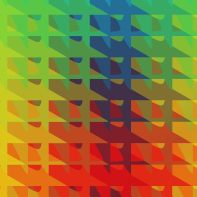
\includegraphics[width=.9\textwidth]{random_art/random_art1.jpg}
    \endminipage
    \minipage{0.32\textwidth}
        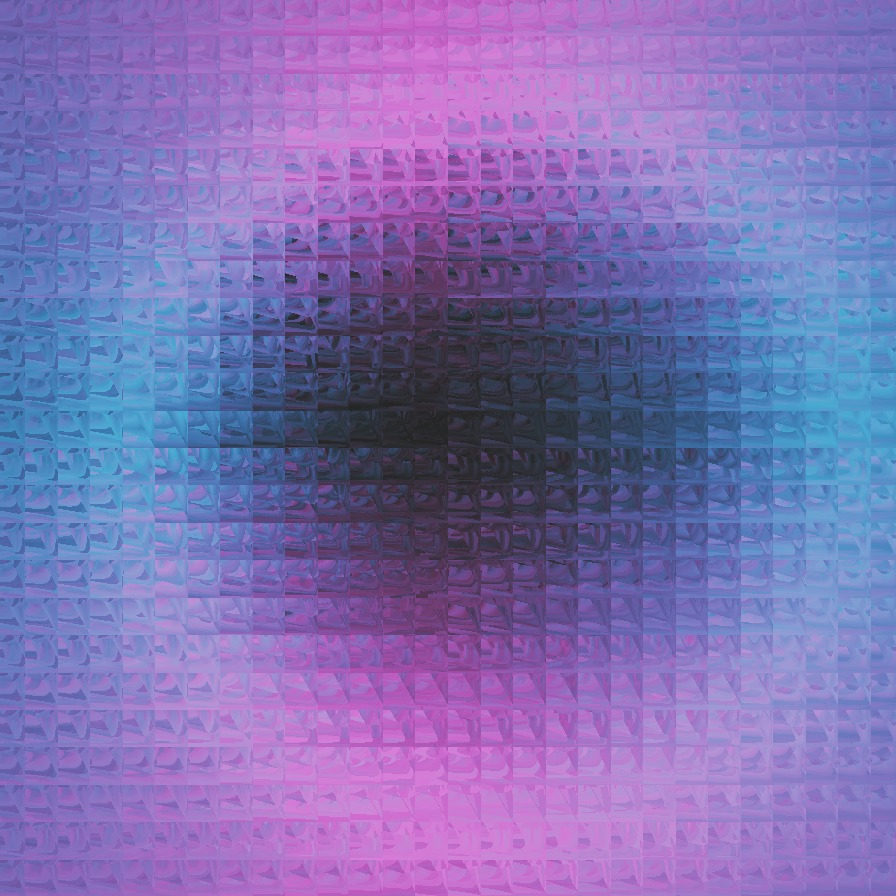
\includegraphics[width=.9\textwidth]{random_art/random_art2.jpg}
    \endminipage
    \minipage{0.32\textwidth}
        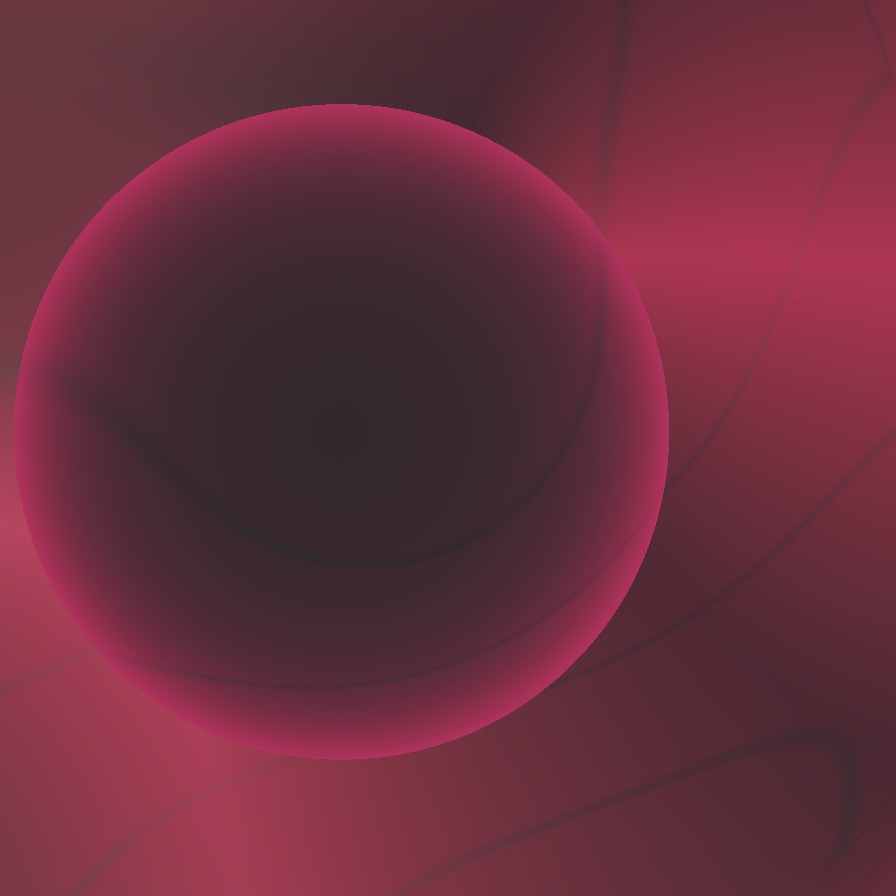
\includegraphics[width=.9\textwidth]{random_art/random_art3.jpg}
    \endminipage
    \caption{Random Art examples}
    \label{fig:randomArt}
\end{figure}

\textbf{Flag}. Flag is a visual hash scheme proposed by \textbf{C. Ellison} and \textbf{S. Dohrmann}\cite{ellison2003public}. Flag consists of four coloured strips with $2^n$ number of possible colours in each strip. 

\textbf{T-Flag}. T-Flag is an attempt to improve on the previously mentioned Flag \cite{lin2010spate}. Improvements include twice the number of coloured blocks with a choice of eight colours. The authors claim the choice of colours are ``colourblind proof''.

\textbf{Flag-Ext}. Flag Extended is the proposed scheme assessed in the paper by \textbf{H. Hsiao \textit{et al.}}\cite{hsiao2009study}. Flag-Ext aims, again, to improve on flag by reducing the number of blocks while adding 8 possible shapes.

Figure \ref{fig:flag} contains an example of each version of Flag discussed.

\begin{figure}[h!]
    \centering
    \minipage{0.32\textwidth}
        
\includegraphics[width=.9\textwidth]{flag/Flag.png}
        \caption{Flag}
    \endminipage
    \minipage{0.32\textwidth}
        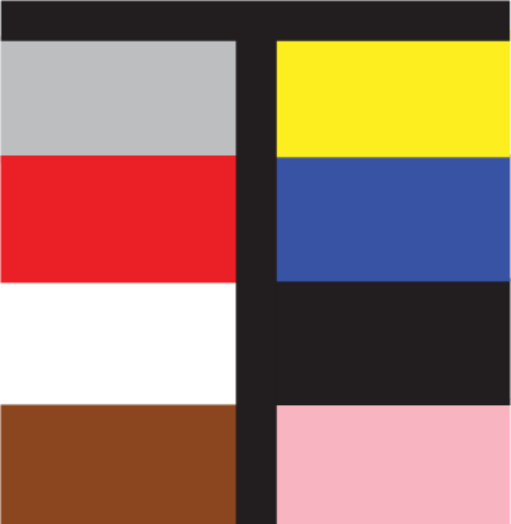
\includegraphics[width=.9\textwidth]{flag/T-Flag.png}
        \caption{T-Flag}
    \endminipage
    \minipage{0.32\textwidth}
        
\includegraphics[width=.9\textwidth]{flag/Flag-ext.png}
        \caption{Flag Ext}
    \endminipage
    \caption{Variations of Flag}
    \label{fig:flag}
\end{figure}

\textbf{OpenSSH}. OpenSSH Visual Host Key is an ASCII based graphical scheme used in MiTM detection when connecting to SSH servers. The image is generated by the movement of the central marker across a grid. Every 2-bits of the generated MD5 hash defines the diagonal direction of movement. For example, if the first 2-bits are \verb|11|, the marker moves South East. The different characters are determined by the number of times the marker is present in that index, for example, if the maker is present on a square 4 times the character is an equals sign (\verb|=|).

\textbf{Unicorns}\footnote{\url{https://unicornify.pictures/}}. Unicorns can be considered an example of an ``Avatar'' graphical scheme. The provided hash changes aspects of the image, such as background colour, horn length and colour of the Unicorn's mane.

\textbf{Vash}\footnote{\url{https://github.com/thevash/vash}}. Vash is similar to that of unicorns, where the hash determines specific characteristics of the image. Vash claims to have $\approx 5,438$ bits of entropy.

\begin{figure}[h!]
    \centering
    \minipage{0.32\textwidth}
        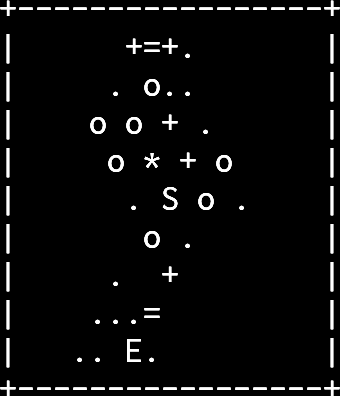
\includegraphics[width=.9\textwidth]{graphical/openssh.png}
        \caption{OpenSSH Visual Host Key}
    \endminipage
    \minipage{0.32\textwidth}
        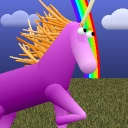
\includegraphics[width=.9\textwidth]{graphical/unicorn.png}
        \caption{Unicorn}
    \endminipage
    \minipage{0.32\textwidth}
        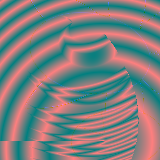
\includegraphics[width=.9\textwidth]{graphical/vash.png}
        \caption{Vash}
    \endminipage
    \caption{Examples of alternative graphical encoding schemes}
\end{figure}

Research in this area has taken these various encoding schemes and compared their fallibility to impersonated attacks. The main elements of comparison have been the ``accuracy of attack detection" and ``time to compare." In this paper, these are considered the metrics of ``security'' and ``usability,'' respectively.

\subsection{Similarity Metrics}
\label{sec:similarity_metric}
A similarity metric is an algorithm designed to determine if two words are phonetically a match. For example, the words "THEIR" and "THERE" is a match, whereas the words "DARK" and "PRINCIPLE" are not phonetically matching. This section provides a base explanation of important phonetic algorithms relevant in this project.

\subsubsection*{Soundex}
\label{sec:soundex}
One of the earliest examples of a phonetic algorithm is known as Soundex. It was initially designed for phonetically indexing names alongside detection of transposed letters in spelling mistakes. 

Soundex produces a four-digit code for each word assessed.
The first letter of the word is retained alongside the removal of all of \verb|a|, \verb|e|, \verb|i|, \verb|o|, \verb|u|, \verb|y|, \verb|h| and \verb|w|. The remaining letters are then mapped to numbers. These mappings are displayed in Figure \ref{fig:soundexMap}.

\begin{figure}[h!]
    \centering
    \begin{BVerbatim}
b, f, p, v               1
c, g, j, k, q, s, x, z   2
d, t                     3
l                        4
m, n                     5
r                        6
    \end{BVerbatim}

    \caption{Soundex mappings of letters to numbers}
    \label{fig:soundexMap}
\end{figure}

Due to the fixed length and limited digit set the initial concerns from this design is the limited number of combinations. There are a total of 5616 codes due to 26 initial letters and three digits of 6 values ($26 * 6^3$).
The limited combinations result in matches of limited quality.

Further issues posed in \cite{patman2001soundex} are discussed below and show the further deficiencies of Soundex in a dictionary word matching context. 

\begin{enumerate}
    \item \textbf{Dependency on the first letter:} Soundex cannot match words together if their first letters are different, meaning, for example, the words "KORBIN" and "CORBIN" are considered non-matching. 

    \item \textbf{Silent consonants.} Soundex does not have logic embedded to deal with silent consonants.

    \item \textbf{Poor precision.} Due to the previously discussed point of a limited code space. \cite{patman2001soundex} re-iterates this point but in the context of name matching where Soundex's poor performance was demonstrated. Soundex only gained and overall accuracy of 36.37\% when matching names within a provided database.
\end{enumerate}

\subsubsection*{NYSIIS}
\label{sec:nysiis}
The New York State Identification and Intelligence System (NYSIIS) phonetic code was created for the phonetic matching of American names. The motivation for its inception was mostly due to the presence of Hispanic names in the American based databases (this was an aspect Soundex was known to have low accuracy with). 

It also allows for variable-length codes and, thus, allows the applicability of the application to increase due to it not confronting the limited code issue of Soundex. It was in use right up until the end of 1998 within various US Government departments.

\subsubsection*{Metaphone}
\label{sec:metaphone}
Metaphone was invented by Lawrence Philips in 1990\cite{philips1990hanging} in response to the deficiencies in Soundex. It improves on Soundex by including information around inconsistency and variation in English spelling in an attempt to create a more accurate phonetic representation.

\subsubsection{Levenshtein Distance}
\label{sec:leven}
Levenshtein distance is a string metric designed to measure the `distance' between two strings. It is merely the number of single-character edits (insertions, deletions or substitutions) required to reach the other string.

An example distance between \verb|trace| and \verb|place| would be the substitutions of the first to letters, from \verb|tr| to \verb|pl|, meaning the two strings have a Levenshtein distance of 2.

\subsubsection{Phonetic Vectors}
\label{sec:phonetic_vectors}
Phonetic Vectors is a unique addition to the chosen set. Created by Allison Parrish in 2017\cite{parrish2017poetic}, Phonetic vectors is as the name suggests the vectorisation of the phonetics of a word.

Phonetic features are used in this work as a way to compare the similarity of phonemes. Phonemes are the phonetic elements that construct a word. For example, the word "RING" translated into the phonemes \verb|/R IH NG/|. 

Extensive prior work has gone into producing models of features that map to phonemes \cite{chomsky1968sound}\cite{ladefoged1969measurement}\cite{bradlow2010perceptual}. Features, therefore, are an attempt at mapping the varying and inconsistent rules around the pronunciation of the English language. The vectors were created using lists phonemes from the CMU Pronouncing Dictionary and mapping them to possible features.

\begin{table}[!htb]
    \tiny
    \begin{minipage}{.33\linewidth}
        \centering
        \begin{tabular}{ll}
            Phone & Features \\
            \hline
            AA & bck, low, unr, vwl \\
            AE & fnt, low, unr, vwl \\
            AH & cnt, mid, unr, vwl \\
            AO & bck, lmd, rnd, vwl \\
            AW & bck, cnt, low, rnd, smh, unr, vwl \\
            AY & cnt, fnt, low, smh, unr, vwl \\
            B & blb, stp, vcd \\
            CH & alv, frc, stp, vls \\
            D & alv, stp, vcd \\
            DH & dnt, frc, vcd \\
            EH & fnt, lmd, unr, vwl \\
            ER & cnt, rzd, umd, vwl \\
            EY & fnt, lmd, smh, unr, vwl
        \end{tabular}
    \end{minipage}%
    \begin{minipage}{.33\linewidth}
        \centering
        \begin{tabular}{ll}
            Phone & Features \\
            \hline
            F &  frc, lbd, vls \\
            G &  stp, vcd, vel \\
            HH & apr, glt \\
            IH & fnt, smh, unr, vwl \\
            IY & fnt, hgh, unr, vwl \\
            JH & alv, frc, stp, vcd \\
            K &  stp, vel, vls \\
            L &  alv, lat \\
            M &  blb, nas \\
            N &  alv, nas \\
            NG & nas, vel \\
            OW & bck, rnd, smh, umd, vwl \\
            OY & bck, fnt, lmd, rnd, smh, unr, vwl
        \end{tabular}
    \end{minipage} 
    \begin{minipage}{.33\linewidth}
        \centering
        \begin{tabular}{ll}
            Phone & Features \\
            \hline
            P & blb, stp, vls \\
            R & alv, apr \\
            S & alv, frc, vls \\
            SH & frc, pla, vls \\
            T & alv, stp, vls \\
            TH & dnt, frc, vls \\
            UH & bck, rnd, smh, vwl \\
            UW & bck, hgh, rnd, vwl \\
            V & frc, lbd, vcd \\
            W & apr, lbv \\
            Y & apr, pal \\
            Z & alv, frc, vcd \\
            ZH & frc, pla, vcd \\
        \end{tabular}
    \end{minipage} 
    \caption{Phonemes to feature mapping table}
    \label{tab:features}
\end{table}

Table \ref{tab:features} contains the mappings used in \cite{parrish2017poetic} to create the phonetic feature lists.
Using this with all 133,852 entries in version 0.7b of the CMU Pronouncing Dictionary, 949 unique properties were produced overall. 

The author then performed principal components analysis\footnote{Details regarding this process are outside the scope of the project. Please, however, if interested please refer to this resource: \url{http://setosa.io/ev/principal-component-analysis/}} on the unique properties to reduce them down to 50.

This metric allows for a unique set of actions to be performed on the phonetic output. Not only does this metric allow the user to measure \textit{dissimilarity} (as opposed to the similar-or-not method of the alternatives) the continuous nature of the value allows mathematical operations to be performed on the output. An example shown in \cite{parrish2017poetic} was the addition of word vectors.

\begin{table}[!htb]
    \centering
    \begin{tabular}{cll}
        No & Operation & Result \\
        \hline
        1  & $Vec(\verb|sub|) + Vec(\verb|marine|)$ & \verb|submarine| \\
        2  & $Vec(\verb|miss|) + Vec(\verb|sieve|)$ & \verb|missive| \\
        3  & $Vec(\verb|fizz|) + Vec(\verb|theology|)$ & \verb|physiology| \\
    \end{tabular}
    \caption{Examples of vector addition}
    \label{tab:vectorAdd}
\end{table}

For example, the addition of vectors can be seen in Table \ref{tab:vectorAdd}. This works for any mathematical operation with examples like multiplication allowing the `tinting' of words with a phonetical theme.



\section{Literature Review}
This section discusses the current research around the proposed topic.

The organisation of the section is as follows:

\begin{itemize}
    \item \textbf{Authentication ceremony performance} \\
    This section explains the current research on the performance of various encoding schemes and methods of comparison, alongside an assessment of the literature's experimental design.

    \item \textbf{Encoding schemes} \\
    The following section then discusses research around the design of an encoding scheme. The focus of the section is the technical details regarding the creation and design of schemes. 

    \item \textbf{Attacks on encoding schemes} \\
    The final section discusses literature that investigates the creation of actual attacks against encoding schemes.
\end{itemize}

\subsection{Authentication ceremony performance}

\subsubsection*{Encoding scheme performance}
Results 
from the literature consistently show the effectiveness of language-based encodings such as Words or Sentences with accuracies ranging up from 94\% \cite{dechand2016empirical}\cite{tan2017can}\cite{kainda2009usability}. In all cases, these were the best schemes from the sets assessed. The exception to this is the work performed by \textbf{H. Hsiao \textit{et al.}}\cite{hsiao2009study} in 2009 with Words achieving an abnormal accuracy of 63\%.
\\\\
Aside from textual representations were graphical schemes. As explained in Section \ref{sec:encodingSchemes}, the primary graphical schemes assessed by the literature were: Random Art, Flag, T-Flag, Vash, OpenSSH Visual Host Key and Unicorns. These schemes had mixed accuracy with ranges as large as 50\% - 94\% in work by \textbf{Hsiao \textit{et al.}}\cite{hsiao2009study}. The only other paper assessing graphical representations was the work of \textbf{Tan \textit{et al.}}\cite{tan2017can}, where they also achieved mixed results with accuracies ranging from 46\% to 90\%.
\\
\begin{table}[h!]
    \makebox[\textwidth][c]{
        \begin{tabular}{c|ccccc}
    \toprule
    \textbf{Scheme} 
    & Hsu-Chun\cite{hsiao2009study}      
    & Kainda\cite{kainda2009usability}      
    & Dechand\cite{dechand2016empirical}
    & Tan\cite{tan2017can}      
    \\\hline
    Hexadecimal     &           &           & 11.20   & 9.00\\
    Numerical       &           & 6.00      & 10.60   & 9.00\\
    Base32          & 3.51      & 6.00      & 10.20   & \\
    Words           & 4.63      & 7.00      & 8.70    & 7.00 \\
    Scentences      &           & 11.00     & 12.30   & 8.00 \\
    Chinese Symbols & 5.01   &           &         & \\
    Japanese Symbols& 5.07   &           &         & \\
    Korean Symbols  & 4.92   &           &         & \\
    \midrule
    Random Art	     & 3.21   &&&&\\
    Flag    	     & 4.28   &&&&\\
    T-Flag  	     & 4.00   &&&&\\
    Flag Ext.	     & 4.02   &&&&\\
    OpenSSH`         &&&& 5.00 &\\
    Unicorns         &&&& 3.00 &\\
    Vash             &&&& 3.00 &\\
    \bottomrule
\end{tabular}
    }%
    \caption{Average comparison time (seconds) for the encoding schemes}
    \label{tab:times}
\end{table}
\\
In terms of usability of graphical schemes, the literature concurred on their high usability. The comparison speed of these schemes were all among the quickest (See Table \ref{tab:times} for an overview of timings). Other work also indirectly agreed with graphical encodings having significantly quicker comparison times compared to non-graphical schemes \cite{dechand2016empirical, kainda2009usability}.
In terms of research into the performance of graphical schemes, the literature does not contain an extensive review with only two papers available. There is also no overlap in the schemes assessed with each paper reviewing a unique set. This area is, therefore, a promising candidate for further research.

One unique paper in this research area was the work by \textbf{M. Shirvanian, N. Saxena and J. J. George}\cite{shirvanian2017pitfalls} produced in the context of secure messaging pairing. This paper was unique for several reasons. First was the consideration for ``remote-vs-proximity'' pairing where this is the first consideration of this aspect found in the literature. There is room for further research to compare encoding schemes in the context of ``remote-vs-proximity.'' Another unique aspect was the end-to-end encryption context of the study.

The findings from the paper showed a high false-negative rate for all the schemes in a remote setting. This consideration is also missing from the literature. Alongside this, results for usability were lower in a remote setting for all the schemes. The author, however, comments on the expected nature of this result.\\
Images were identified as being the most secure method of authentication in the remote setting but voted as the method with the worst usability. This conclusion is highly inconsistent with all other work in this area. However, this could be due to the unique setting of remote verification, resulting in distinct results from user studies. Without further work in this area, it is difficult to validate these results conclusively.

Alongside this, it was shown in work by \textbf{H. Hsiao \textit{et al.}}\cite{hsiao2009study} that age and gender do not affect the accuracy of the scheme. However, younger participants were considerably faster. Furthermore, findings also showed that language comprehension helped in discerning small differences between schemes encoded in Chinese, Japanese, Korean, or English. Subsequently, knowledge of the language did not assist in differentiating more significant changes in the schemes as these had high accuracy regardless. These were unique considerations. Further work could aim to corroborate these conclusions.

\begin{table}[h!]
    \centering
    \resizebox{.8\textwidth}{!}{%

        \makebox[\textwidth][c]{
            \begin{tabular}{c|ccccc}
    \toprule
    \textbf{Scheme\footnote{All values have been rounded to the nearest whole percentage}} 
    & Hsu-Chun\cite{hsiao2009study}      
    & Kainda\cite{kainda2009usability}      
    & Dechand\cite{dechand2016empirical}
    & Tan\cite{tan2017can}      
    & M. Shirvanian\cite{shirvanian2017pitfalls}
    \\\hline
    Hexadecimal     &        &        & 90\% & 79\% &            \\
    Numerical       &        & 100\%  & 94\% & 65\% & 97\%       \\
    Base32          & 86\%   & ~~90\% & 92\% &      &            \\
    Words           & 63\%   & 100\%  & 94\% & 94\% &            \\
    Scentences      &        & 100\%  & 97\% & 94\% &            \\
    Chinese Symbols & 59\%   &        &      &      &            \\
    Japanese Symbols& 57\%   &        &      &      &            \\
    Korean Symbols  & 54\%   &        &      &      &            \\
    \midrule
    Random Art	     & 94\%   &&&&\\
    Flag    	     & 50\%   &&&&\\
    T-Flag  	     & 85\%   &&&&\\
    Flag Ext.	     & 88\%   &&&&\\
    OpenSSH`         &&&& 90\% &\\
    Unicorns         &&&& 46\% &\\
    Vash             &&&& 88\% &\\
    \bottomrule
\end{tabular}
        }%
    }
    \caption{Overall accuracy of correct comparison for the encoding schemes assessed}
    \label{tab:results}
\end{table}

Tables \ref{tab:times} \& \ref{tab:results} contain the accuracy results of all papers assessed; this is to aid in visual comparison. Each paper used a different metric for measuring accuracy. Therefore, all results have been translated into ``overall accuracy.''. For example, if a paper presented "security failures" or "attack success rate" of 5\%, the overall accuracy of the scheme is 95\%.

\subsubsection*{Methods of comparison performance}

Method of comparison is the way a user compares the encoding schemes output. The most common example and the one used as default is ``Compare-and-Confirm'' (CaC). CaC, as the name suggests, is the \textit{comparison} of two fingerprints on different devices or mediums that are then \textit{confirmed}. 

Aside from ``Compare-and-Confirm'' (CaC), there is ``Compare-and-Select'' (CaS) and ``Compare-and-Enter'' (CaE). CaS is the method where one device displays the fingerprint, and the other user is provided with several options. The user then has to choose the correct value from the list of candidates. If there is no match, the user must deny the connection attempt. The creation of CaS was due to concerns that CaC would be ``too easy'' for users leading to complacency and errors\cite{uzun2007usability}. The design of CaE is for scenarios where both devices might not have a display, i.e., pairing between a phone and a keyboard. One device displays the checksum. This checksum is then entered into the other device. The first device then compares the entered string and checks for a match.

Research has assessed the performance of these schemes and how they affect the security of the authentication ceremony. The literature agrees on CaC being the best overall scheme to compare fingerprints \cite{tan2017can}\cite{uzun2007usability} with CaS highlighted for its poor security and usability. CaE has had conflicting results. \cite{uzun2007usability} discarded it after one round due to ``poor usability.'' However, \cite{tan2017can} considered it the best method overall for usability and security. These conflicting results, therefore, show polarisation in the results of CaE. However, this could be due to the different overall use-cases of the studies. Validation of results from either study would, therefore, be an area of additional study.

\subsubsection*{Experimentation methodology comparison}
To further look into the validity of previously discussed results, it is necessary to asses how the respective studies reached their conclusions. Areas for consideration are scheme entropy, attacker strength, and participant demographics.

The starkest limitations of the literature are the range of participants and encoding entropy. The worst studies tested only 22-bits of entropy. This lack of entropy makes it challenging to compare results directly. One of the papers this most effects is the early work by \textbf{H. Hsiao \textit{et al.}}\cite{hsiao2009study}  where their highest entropy is 28-bits. This level of entropy was inadequate even at the time of publication. There is an attempt by the authors' to address this issue in the later stages of the paper where they write: \textit{``[...] increasing entropy is not a solution because it sacrifices usability and accuracy. With more entropy, representations will contain longer sequences of characters or more minute details which will lead to increased time and errors during comparisons.''}. This statement is backed up with no empirical evidence, and the authors fail to consider how the low entropy would affect the overall security of the schemes.

Attacker strength is also another metric used to compare results concluded by each paper. Some papers failed to address their attacker strength consideration directly, but the overall strength has been inferred from the changes made to their schemes. For example, if they decided to change a single character in a 40-digit (160-bit) SHA-1 hex digest, they are indirectly stating that the attacker can control 39-digits (156-bit). To achieve this, the attacker would have to compute $2^{156}$ SHA-1 compressions to find a key match.
In the literature, this element ranged from $2^{28}$ to around $2^{242}$. However, this has some relation to the size of the encoding schemes used. This substantial range makes it challenging to compare and confer results confidently. 
Further work could exclusively look into the effects that attacker strength has on the success of attacks. Moreover, all the papers assessed failed to fully consider the feasibility of attacks in terms of computer and storage requirements. 

All of the studies considered demographical data when presenting their results. Their average ages were all around $\sim35$ years old with the majority of participants educated with at least a bachelor degree. Alongside, the equal split between male and female participants.

One consideration of note is that made by \textbf{S. Dechand \textit{et al.}}\cite{dechand2016empirical} where they briefly consider medical conditions such as ADHD and reading or visual disorders and the way they affect the comparison's effectiveness. The results highlight a slight reduction in overall accuracy; however, due to their small sample size, the results cannot be considered conclusive. This aspect is unique to all literature assessed. Further work would be required to produce conclusive results. Therefore, highlighting a gap in the literature.

One glaring issue with the demographical health of the study by \textbf{E. Uzun, K. Karvonen} and \textbf{N. Asokan}\cite{uzun2007usability} is the use of two entirely different groups of participants. Not only were their demographics different, but they were from different countries (America and Finland). Different cultures contain inherent biases and assumptions. Changes were made pragmatically regarding the results from the first round of 40 participants. These were then re-assessed, alongside the direct comparison of results. This aspect casts vast doubts on the validity of the results with no consideration made by the authors to control external factors that may affect the performance of the method of comparison.

Hexadecimal and numerical schemes were not included as encoding schemes in work by \textbf{H. Hsiao \textit{et al.}}\cite{hsiao2009study} (some of the most widespread encoding schemes). The justification was the schemes similarities to Base32  alongside "well-known deficiencies". This point was provided with no further justification. Moreover, it is also inconsistent with available research, for example, in \textit{``Empirical Study of Textual Key-Fingerprint Representations''}\cite{dechand2016empirical} it was shown numerical representations performed significantly better than that of Base32.

\begin{table}[h!]
    \centering
    \resizebox{.8\textwidth}{!}{%
        \makebox[\textwidth][c]{
            \begin{tabular}{c|ccccc}
    \toprule
                        & Hsu-Chun\cite{hsiao2009study}      
                        & Kainda\cite{kainda2009usability}      
                        & Dechand\cite{dechand2016empirical}
                        & Tan\cite{tan2017can}      
                        & M. Shirvanian\cite{shirvanian2017pitfalls}
                        \\\hline
    Attacker Strength\footnote{Some attacker strengths are estimations due to the lack of quantification in some papers.}   
    & $\sim2^{28}$  & $\sim2^{40}$ & $2^{80}$ & $2^{60}$ & $\sim2^{242}$ \\
    Entropy Range       & 22-28 bits    & 20-40 bits   & 122 bits & 128 bits & 160-256 bits  \\
    No\degree  ~Participants     & 436           & 30           & 1047     & 661      & 25            \\
    \bottomrule
\end{tabular}
        }%
    }
    \caption{Paper attribute comparison}
    \label{tab:attacker}
\end{table}

Table \ref{tab:attacker} has been provided to compare the different aspects of the papers' parameters visually. It can be seen from the table the substantial ranges in participant size, entropy and attacker strength.

\subsubsection*{Conclusion}
Overall, this review has identified several key areas suitable for further work.
The first is the performance assessment of graphical encoding schemes. Recreation of pre-existing results from \cite{hsiao2009study}\cite{tan2017can} is required to corroborate current conclusions and validate results.
Another gap in the research is the consideration into the utilisation of encoding schemes in realistic conditions, i.e. ``remove vs proximity." This topic was initially covered by \cite{shirvanian2017pitfalls}, but their scope was limited. 

Further work, therefore, could increase the scope and touch upon a large number of schemes in these settings. The final aspect for further work is the limited consideration into the feasibility of attacks on encoding schemes. All of the papers assessed simulated attacks and had minimal consideration for their execution. Therefore, further work could delve
into the implementation and feasibility of such attacks.

\subsection{Encoding schemes}
Another area of research is investigations into the actual physical encodings of the hash digest. This section discusses the current research on the creation and security of actual encoding schemes. The technical and operation details are outside the scope of this literature review. Therefore, minimal attention is allocated to these areas.

Some of the oldest preliminary work into visual encoding schemes is by \textbf{A. Perrig} and \textbf{D. Song}\cite{perrig1999hash} in the creation of their scheme ``Random Art" in 1999. The motivation for creating such a scheme was the perceived flaws in the ways humans verify and compare written information. As mentioned in previous sections, visual encoding schemes have been shown to have mixed success, with low security being one of their most alarming flaws. This research laid the foundation for further work in analysing the security of visual encoding schemes.

Further research into the creation of unique visual hash schemes has been performed by \textbf{C. Ellison} and \textbf{S. Dohrmann}\cite{ellison2003public} (Flag), \textbf{Yue-Hsun Lin \textit{et al.}}\cite{lin2010spate} (T-Flag) and work by \textbf{M.  Olembo \textit{et al.}}\cite{olembo2013developing}. Each publication has provided a new way  to represent a key fingerprint visually. Alongside the academic literature, there are informally presented methods of visual fingerprints such as Unicorns\footnote{\url{https://unicornify.pictures/}} and Robots\footnote{\url{https://github.com/e1ven/Robohash}}. This list is by no means exhaustive but is used to depict the amount of research and work invested into graphical hash representations.

One paper of note is the preliminary work performed by \textbf{D Loss \textit{et al.}}\cite{loss2009drunken} in their \textit{``An analysis of the OpenSSH fingerprint visualisation algorithm''} where  they aimed to spur on further research with their initial findings into the security of the OpenSSH scheme. The authors claim that the use of the algorithm in OpenSSH is only heuristically justified, and a more formal proof is required.\\
The paper proposed several ways to generate similar fingerprints. The methods proposed were: Naive brute force, Graph Theory, and brute force of a full visual set. They were only able to produce only initial results and have proposed a large amount of potential further work. Since the paper's publication in 2009, there seems to have been no research building on the work of the authors.

Minimal research has also focused on elemental textual fingerprint representations and their security. Work by \textbf{A. Karole} and \textbf{N. Saxena}\cite{karole2009improving} looked into ways to improve the security of a textual representation. This research aim was to improve the secure device pairing process of comparing two numerical values. The devices used (Nokia 6030b; Mid-range devices at the time of publication) and the SAS (Short Authentication String) compared results in findings that are not directly applicable in a fingerprint comparison context. 

A more specific subsection of textual fingerprints is the use of words and sentences to encode hash digests. Some of the first work in this area was by \textbf{Juola} and \textbf{Zimmermann} \cite{juola1996whole}. Their work aimed to produce a word list where phonetic distinctiveness was prioritised. Each word is mapped to a single byte. The unique aspect of the word list is the separation of ``even'' and ``odd'' words. Even byte indices are sampled from the even-list and odd indices from the odd-list. This technique effectively creates two sub-word lists.  A genetic algorithm was used to maximise linguistic distance. The paper also includes a study on effective measures of ``linguistic distances'' of words and provided an in-depth discussion into these areas.

Overall the paper provides a foundation for formalising the creation of useful wordlists. A limitation is the lack of empirical data gathered on the performance. However, this was later evaluated in work by \textbf{S. Dechand \textit{et al.}}\cite{dechand2016empirical} and shown to be an effective encoding scheme.

Other research of note is work by \textbf{M. Goodrich \textit{et al.}}\cite{goodrich2006loud} called \textit{Loud and Clear: Human-Verifiable Authentication Based on Audio}. As the name suggests, the authors were researching ways to improve current methods of secure device pairing. The unique aspect of this work is the use of a Text-to-Speech system reading out syntactically correct English sentences. MadLibs\footnote{\url{https://en.wikipedia.org/wiki/Mad\_Libs}} was the base for these sentences. MadLibs is where static placeholders are replaced with a member from a list of potential words.\\
This work is an extension to work performed by \textbf{Juola} and \textbf{Zimmermann}\cite{juola1996whole} as they aimed to emulate the techniques used in PGPfone. The paper's findings are limited by the lack of empirical data backing up claims made by the author the performance of the system, and security is only theoretically assessed.

Aside from this research, there have been further informal implementations of fingerprint encodings -- The first being by \textbf{Michael Rogers}\footnote{\url{https://github.com/akwizgran/basic-english}}. Rogers' implementation is a program designed to map fingerprints to pseudo-random poems. This implementation was again, empirically evaluated by \textbf{S. Dechand \textit{et al.}}\cite{dechand2016empirical}. Earlier work by \textbf{N. Haller} with the S/KEY\cite{haller1995s} shows the implementation of a system designed to represent a hash as a series of six short words. However, this system is designed for a one-time-password purpose and only provides word mappings for basic human usability of the password and not within a fingerprint verification context. Therefore, the wordlist has not been designed with pronounceability in mind.
Aside from this research, there have been further informal implementations of fingerprint encodings  The first being by \textbf{Michael Rogers}\footnote{\url{https://github.com/akwizgran/basic-english}}. Rogers' implementation is a program designed to map fingerprints to pseudo-random poems. This implementation was again, empirically evaluated by \textbf{S. Dechand \textit{et al.}}\cite{dechand2016empirical}. Earlier work by \textbf{N. Haller} with the S/KEY\cite{haller1995s} shows the implementation of a system designed to represent a hash as a series of six short words. However, this system is designed for a one-time-password purpose and only provides word mappings for basic human usability of the password and not within a fingerprint verification context. Therefore, the wordlist has not been designed with pronounceability in mind.

\newpage
\subsubsection*{Pretty Easy Privacy}
\label{sec:pep}
A very recent implementation of a word list can be found in Pretty Easy Privacy (\pep) implementation of TrustWords\footnote{\url{https://tools.ietf.org/html/draft-birk-pep-trustwords-03}}. \pep is a data encryption system that utilises PGP encryption to provide E2EE on all common channels of communication such as email or SMS. The embedded design principles state that above all the systems should be easy to install, use and understand.

\begin{wrapfigure}{r}{6cm}
    \centering
    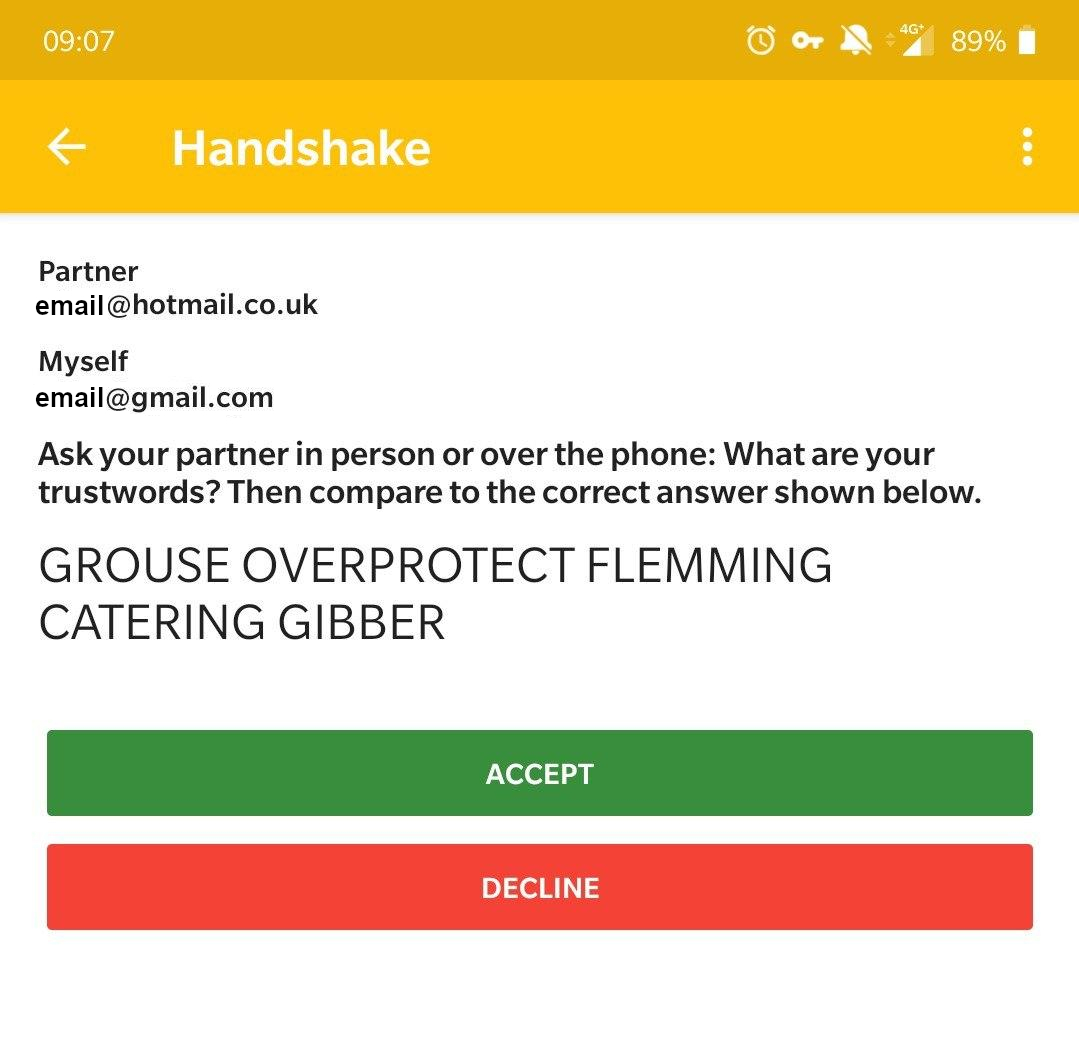
\includegraphics[scale=0.15]{trustwords/trustword_handshake.jpg}
    \caption{Trustword fingerprint verification}
    \label{fig:trustwords}
\end{wrapfigure}

\pep deals with the threat of MiTM attacks by having users compare the respective key fingerprints encoded as a set of words. Figure \ref{fig:trustwords} shows the \pep Android implementation of Trustwords. The users then authenticate the words on an OOB (Out of Band) channel such as a phone call or in-person communication. If both users decide the words match, they accept or decline respectively.

The unique aspect of TrustWords is its mapping of a single word to 16-bits. If compared to alternative literature, this is the highest number of bits-per-word seen. Full mappings (no duplication of words) would, therefore, require $2^{16}$ words in the dictionary. This number of words is arguably higher than most users' vocabulary. This deviation from the norm has not been currently backed up by research. 

\begin{wrapfigure}[11]{l}{5cm}
    \centering
    \begin{BVerbatim}
    [...]
52127 ZYGOTE
52128 ZYGOTIC
52129 ZYMURGY
52130 AACHEN
52131 AARDVARK
52132 AAREN
    [...]
    \end{BVerbatim}
    \caption{Re-mapping position}
    \label{fig:remap}
\end{wrapfigure}

Alongside the abnormally high number of words, the design choice to exclude slang and profanities from the English Trustword dictionary requires dual-mapping of a section of words. Approximately 13633/65536 (20.8\%) of words are re-mapped in the dictionary, leaving 51903 unique words. The re-mapping is performed on an alphabetical loop. Figure \ref{fig:remap} shows the position in the dictionary where this occurs.

\newpage

Moreover, the primary RFC documentation remains in a draft stage and states: \textit{``It is for further study, what minimal number of words (or entropy) should be required.''}. These aspects highlight a substantial gap in the current literature.

\subsubsection*{Conclusion}

In conclusion to this topic, the current research has primarily focused on the research and creation of visual representations. Research for textual fingerprints is fragmented and incomplete with work \textbf{Juola} and \textbf{Zimmermann} 
\cite{juola1996whole} and \textbf{M. Goodrich \textit{et al.}}\cite{goodrich2006loud} providing meaningful research to build upon in terms of word and sentence based encodings. The fragmentation of this research leaves room for further work into this topic area. Alongside this, findings from the previous section's research show that human language based encodings provided the best usability and, therefore, should be a target for further research looking to improve upon their security and usability.

\subsection{Attacks on encoding schemes}
This area of research studies ways to physically execute attacks on fingerprint encoding schemes. This topic differs from previously examined work due to a central focus on the implementation details of an attack. Previous work discussed has only simulated the result of respective attacks. Research in this area is scant, with lots of research focusing on the security and prevention of Man-in-the-Middle (MITM) attacks.

Research in 2002 by \textbf{Konrad Rieck}\cite{rieck2002fuzzy} is one the first formalisation of attacks on fingerprint representations. The paper titled \textit{``Fuzzy Fingerprints Attacking Vulnerabilities in the Human Brain''} aimed to look into ways users check hexadecimal encoded OpenSSH fingerprint representations. The author created an elegant way to `weight' essential chunks of the digest. The bytes furthest to the right and left of the digests provided the highest weight. This technique provides a way to score digests and determine the best partial collisions found. For example, with the target fingerprint: \verb|9F23| and partial match \verb|9313| is given a score of 45\% even though only two characters are matching.

The paper contains an implementation with a ``1.2GHz CPU'' being able to obtain 130,000 H/s (With MD5). In comparison to this, a mid-range Intel i5-3320M CPU can today obtain 111,700,000 MD5 H/s. This imbalance shows that the results obtained from the paper are significantly outdated. However, even with the low hash rate, the author was able to obtain some promising results. Figure~\ref{ref:fuzz} contains the best example used.

\begin{figure}[!h]
    \centering
    \verb|TARGET: d6:b7:df:31:aa:55:d2:56:9b:32:71:61:24:08:44:87|
    \verb|MATCH:  d6:b7:8f:a6:fa:21:0c:0d:7d:0a:fb:9d:30:90:4a:87|
    \caption{Best match obtained after a few minutes of hashing}
    \label{ref:fuzz}
\end{figure}

Overall the paper shows an interesting way to create partial fingerprint matches but is not quantified by any empirical evidence gathered on real-world users. 

The only other relevant research on this topic is the work by \textbf{M Shirvanian and N. Saxena}\cite{shirvanian2014wiretapping} 
and their paper: \textit{``Wiretapping via Mimicry: Short 
Voice Imitation Man-in-the-Middle Attacks on Crypto 
Phones''}. Further research in the area of ``human voice impersonation'' has received lots of attention \cite{mukhopadhyay2015all}\cite{chen2017you}\cite{wu2015spoofing}. This paper was chosen over other alternatives due to its specific use of encoding schemes in its evaluation.

In this paper, the authors develop a way to 
impersonate users when authenticating 
Short-authentication-Strings (SAS) in the pairing of 
Crypto-phones. To achieve this impersonation they propose 
two methods: ``Short voice re-ordering attack'' where an 
arbitrary SAS string is recreated by re-ordering voice snippets 
obtained from eavesdropping a previous connection
and ``Short voice morphing attacks'' whereby the use of 
previously eavesdropped audio snippets the attacker can
morph their voice to match that of the victim. With 
these methods, they aimed to attack encodings of Numbers, 
PGP word list (previously discussed work by \textbf{Juola} and 
\textbf{Zimmermann} \cite{juola1996whole}) and MadLib (\textbf{M. Goodrich 
\textit{et al.}}\cite{goodrich2006loud} work also 
previously discussed). The effectiveness of these attacks 
was evaluated with a study involving 30 participants.

Results from the paper show the effectiveness of these 
methods. Compared to the baseline of the attacker's voice 
replacing the victim, performed with an $\sim$18\% success rate. Morphing gained an overall success rate of 50.58\% and re-ordering a very impressive 78.23\% success rate and showing that these attacks provide an improvement on top of the naive implementation.

One of the most significant limitations addressed by the authors  was the reduction in success rates as the size of the authentication string grew. The morphing and re-ordering  attacks become increasingly ineffective as the user had more time to detect imperfections. The author does not quantify this aspect, and the extent of this degradation is never empirically discussed. Therefore, the results from this study are only practical and applicable in a SAS context.

\subsubsection*{Conclusion}
Overall the literature for this subtopic remains sparse and incomplete. Further suggested work could look into the feasibility of generating partial collisions for all textual representations alongside quantified effectiveness on users. The work would aim to focus on the various physical methods used and their feasibility. This is one area the previous literature has failed to cover and has only theoretically quantified attacker strength without consideration for the actual real-world cost.

\section{Overall Summary}
In summary of the literature gaps discovered; encoding scheme performance requires further work focusing on all graphical schemes to corroborate results made by other work. Furthermore, there is a gap with the assessment of encoding schemes in the context of "remote-vs-proximity" first proposed by \textbf{M. Shirvanian, N. Saxena} and \textbf{J. J. George}\cite{shirvanian2017pitfalls} as it would arguably provide a better simulation of real-world scenarios.

In the context of human demographics and the way they alter the performance of the schemes; further research is required into how the fluency of languages affects authentication ceremony. This further work would be a continuation of the initial work by \textbf{H. Hsiao \textit{et al.}}\cite{hsiao2009study} and could allow the creation of schemes that are better suited to specific languages.
Alongside this, there is a research gap in the investigation of how mental impairments affect the performance of a scheme. This aspect is useful due to the number of potential users being affected. For example, 7\% of the population have been identified as having dyslexic tendencies\cite{peterson2012developmental}. This fact means that with a UK population of around 63,000,000\footnote{From the 2011 Census collated by the Office for National Statistics}  4,410,000 people could benefit from encoding schemes designed to work well with dyslexia. Dyslexia, however, is only one of many impairments that could affect a scheme's performance, thus, contributing to the substantial effect further work could have on this area.

Other possible large areas for consideration is the lack of direct consideration for attack strength when assessing the vulnerability of encoding schemes. Issues included the previously discussed wide range of attack strength ($2^{28}$ - $2^{242}$) alongside the lack of consideration at all from the majority of papers. Moreover, the complete lack of computation and storage complexity considerations means this is a prime area for further research as it would improve the applicability of results.

The final significant research gap identified is the lack of justification for the newly created Trustwords. Abnormal design choices (16-bit per word) and its recent creation alongside the shown effectiveness of language-based encodings, such as words makes this a promising area for further research. 
  \chapter{Project Aims}

This chapter defines the selected gaps and the subsequent research questions extracted.

The chosen project aims to asses the security of \pep's minimum recommendation of four Trustwords (As stated in Figure \ref{fig:trustwordsNum}). As discussed in the previous chapter, Trustwords aims to sacrifice security for increased usability. The encoding scheme has been designed to assist this by having  the user compare a reduced set of words. Moreover, issues with the dictionary's design, such as the presence of homophones and dual-mapping of words show the potential for possible vulnerabilities. 

As discussed in the previous chapter, the identified research gap regarding the minimal consideration of attack complexity would be a suitable addition for this project. This choice is due to it providing the ability to asses actual performance and, thus, the actual real-world strength of Trustwords while providing research to a scant area. Therefore, the security assessment is supplemented with complexity considerations alongside an actual implementation of the attack proposed.

\begin{center}
\begin{figure}[h!]
    \centering
        
    \begin{lstlisting}[frame=single, numbers=none]
"Short Trustword Mapping (S-TWM) requires a number of 
Trustwords that MUST retain at least 64 bits of entropy. 
Thus, S-TWM results into at least four Trustwords to be 
compared by the user."
    \end{lstlisting}

    \caption{Most recent RFC security recommendation}
    \label{fig:trustwordsNum}
\end{figure}
\end{center}
By sampling the \pep documentation they have defined the use case of the Trustword handshake: \textit{``A handshake is done by comparing the Trustwords between two users through a separate communication channel (e.g. in person or by phone)''.}\footnote{\url{https://www.pep.security/docs/general\_information.html\#handshake}}. It can be assumed due to the increased globalisation of the planet that the most common handshake occurrence is over the phone, and, therefore, not in person. This is the assumed context of the handshake. This means, to create near-matches, the similarity of words is quantified phonetically instead of visually.

\section{Research Questions}

With the previously discussed points in mind, the following research questions have been proposed.

\begin{enumerate}
    \item  What are the best performing schemes to quantify phonetic similarity?  \label{goal:phoneticSimilarity}

    \item What is the time and computation complexity required to generate a 'similar' keys for a targeted key pair? \label{goal:complexity}
    
    \item What percentage of attacks successfully deceive a user? \label{goal:attackPercentage}

    \item Is the recommended minimum number of four Trustwords enough to provide a basic level of security? \label{goal:numberOfTrustwords}
\end{enumerate}

  \section{Design}

\subsection{Attack Design}
\label{sec:attackDesign}
The propossed attack on Trustwords involves generating ``near-collision'' keys. Near-collision keys are keys composed of a set of words that are deemed a match by the similarity metrics.
\\\\
The attack is designed to target a single pair of users and requires recomputation for each attack target pair. Each pair is split into an "Uncontrolled" or "Controlled" key. Uncontrolled is the receiver of the communication, and, thus, the key cannot be altered. The Controlled key is the one we are attempting to impersonate. It is assumed that there is the ability to replace the Controlled key with the malicious option. The uncontrolled and controlled keys can be swapped around, thus, resulting in the possibility to intercept both directions of communication.
\\\\
When attacking, a similarity metric is used to compute a list of possibilities for each position in the target fingerprint. Completing these steps produces a list of fingerprints that can be inserted into a tool designed to hash a large number of keys and search for matches. This aspect of using an extensive list to search for keys massively reduces the complexity of the search.

In summary, the attack steps are:
\begin{enumerate}
    \item Compute all possible matches using a similarity metric on all words in a dictionary (Only needs performing once).

    \item Select a target and allocate ``Uncontrolled" and ``Controlled" key identification.
    
    \item Calculate all permutations of near-collisions for the key pair and produce a list of near-collision fingerprints.
    
    \item Use a list of near-collision fingerprints in the mass computation of keys to find near-collision keys.

\end{enumerate}

\subsection{GreenOnion Design}

The inspiration for the design of this tool was taken from a tool called Scallion\footnote{\url{https://github.com/lachesis/scallion}}. The proposed tool is called `GreenOnion' and is a re-write of Scallion in C++.  The proposed tool differs from Scallion, most notably in its ability to concurrently search for a large number of keys. This is due to the unique addition of a bloom filter. A bloom filter is a probabilistic data structure that allows efficient checking for the presence of an element in a set. It is effectively a vast array of booleans that state whether an element is present. A pre-defined hashing algorithm decides the index in the array. This process is repeated several times with a set number of hashing algorithms ($k$) to populate the array of length ($m$). To check the presence of an element in the set means hashing the target value and checking the indices returned. This data structure, therefore, has a complexity of $O(k)$ regardless of the number of elements in the set. Due to the use of hashing algorithms, there is the possibility for collisions and, thus, the possibility of false-positives. The data structure, however, does not produce any false-negatives. If the levels of false-positives are controlled (by altering $k$ and $m$), the tool can search through a vast number of potential keys with minimal decrease in speed.

The tool should take two keys as parameters (Uncontrolled/Controlled) and a chosen similarity metric and produce a list of target key fingerprints. This list is then used as a search criterion when searching for keys. To utilise the parallel nature of the GPU to compute the hash of a large number of keys, the tool utilises a GPGPU (General-purpose computing on graphics processing units) framework. OpenCL allows the creation of code chunks referred to as ``kernels'' to be executed concurrently, this provides a massive speed increase compared to the sequential nature of the CPU.
  \chapter{Implementation}
\label{cha:Implementation}

This chapter discusses the implementation details of the project. Instead of explaining all the technical achievements in detail, the most interesting ones are discussed alongside the respective challenges encountered.

\section{GreenOnion}

\subsubsection{General design}
This section briefly discusses the overall technical implementation of GreenOnion alongside a more in-depth discussion into the unique aspect of the tool.

GreenOnion is written in C++. This language was chosen due to its efficiency bonuses over other alternative languages.
The tool begins by generating a 2048-bit RSA key through GPG\footnote{GNU Privacy Guard}. This key is then used to create a hash of all but the final 512-bit block of the key. The final block of the key is left un-hashed due to the presence of the exponent ($e$). This exponent is then incremented to create a new unique key. This technique allows the accelerated generation of new keys due to the reduction in expensive large prime generation. Entropy starvation is an example of a common issue encountered when generating a large number of RSA keys. This process produces valid keys, but with abnormally large exponents, this was deemed suitable due to the short term use-case for these keys. Three bytes are used to represent the exponent giving the potential to create $2^{24} - 1$ extra keys for a single expensive key generation.

The intermediate hash is then loaded on the GPU via an OpenCL kernel. This kernel is designed to increment the exponent, hash the final block, obtain the final fingerprint and check if the fingerprint is present in the provided data structure.

\subsubsection{Bloom filter}

Mass checking of fingerprints is the tool's central ability as it allows for millions of keys to be checked with a minimal amount of overhead. This functionality is achieved through the use of a bloom filter. A bloom filter is a probabilistic data structure that allows efficient checking for the presence of an element in a set. It is effectively a vast array of booleans that state whether an element is present. A pre-defined hashing algorithm decides the index in the array. This process is repeated several times with a set number of hashing algorithms ($k$) to populate the array of length ($m$). To check the presence of an element in the set means hashing the target value and checking the indices returned. This data structure, therefore, has a complexity of $O(k)$ regardless of the number of elements in the set. This is the only data structure that provides this characteristic. This benefit comes at a cost. Due to the use of hashing algorithms, there is the possibility for collisions and, thus, the possibility of false-positives. The data structure, however, does not produce any false-negatives. 

These qualities, therefore, makes it fully suited to this use-case as any fingerprints tagged as ``possibly'' being present in the bloom filter can be followed up with a more expensive hash-table check to determine their actual presence. Therefore, if the levels of false-positives are controlled (by altering $k$ and $m$), the tool can search through a vast number of potential keys without any decrease in speed.

\begin{figure}[h!]
    \centering
    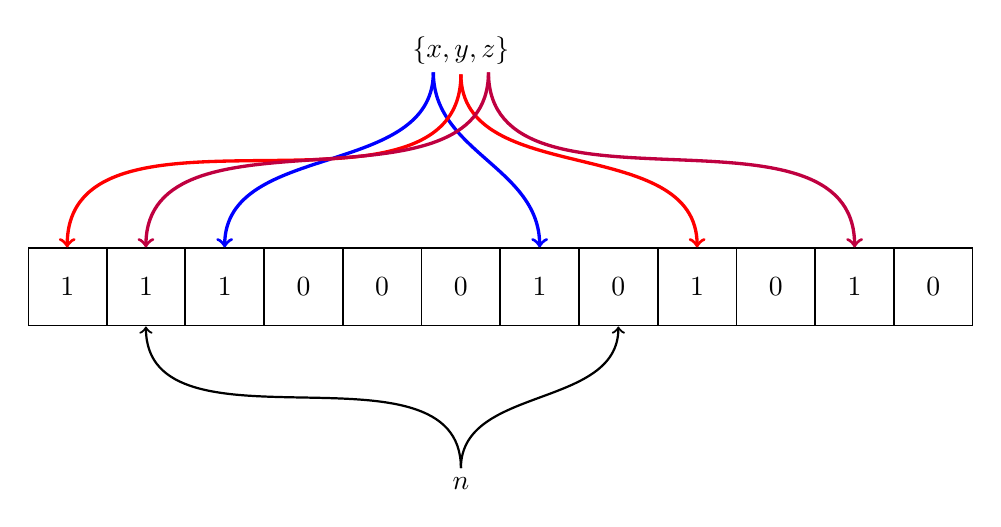
\begin{tikzpicture}[
    square/.style={regular polygon,regular polygon sides=4, minimum size=1.4cm}
]

    \node at (0,0) [square,draw] (box_0) {$1$};
    \node at (1,0) [square,draw] (box_1) {$1$};
    \node at (2,0) [square,draw] (box_2) {$1$};
    \node at (3,0) [square,draw] (box_3) {$0$};
    \node at (4,0) [square,draw] (box_4) {$0$};
    \node at (5,0) [square,draw] (box_5) {$0$};
    \node at (6,0) [square,draw] (box_6) {$1$};
    \node at (7,0) [square,draw] (box_7) {$0$};
    \node at (8,0) [square,draw] (box_8) {$1$};
    \node at (9,0) [square,draw] (box_9) {$0$};
    \node at (10,0) [square,draw] (box_10) {$1$};
    \node at (11,0) [square,draw] (box_11) {$0$};

    \node[] (set) [above of=box_5, yshift=2cm] {$\{x, y, z\}$};
    \node[] (set_x) [left of=set, xshift=0.65cm, yshift=-0.15cm] {};
    \node[] (set_z) [right of=set, xshift=-0.65cm, yshift=-0.15cm] {};
    \node[] (new_set) [below of=set, yshift=-4.5cm] {$n$};

    % X
    \draw [->, very thick, blue] (set_x) to [out=-90, in=90, xshift=2cm] (box_6);
    \draw [->, very thick, blue] (set_x) to [out=-90, in=90, xshift=2cm] (box_2);

    % Y
    \draw [->, very thick, red] (set) to [out=-90, in=90] (box_0);
    \draw [->, very thick, red] (set) to [out=-90, in=90] (box_8);
    
    % Z
    \draw [->, very thick, purple] (set_z) to [out=-90, in=90, xshift=2cm] (box_1);
    \draw [->, very thick, purple] (set_z) to [out=-90, in=90, xshift=2cm] (box_10);

    % N
    \draw [->, thick] (new_set) to [out=90, in=-90, xshift=2cm] (box_1);
    \draw [->, thick] (new_set) to [out=90, in=-90, xshift=2cm] (box_7);
\end{tikzpicture}
    \caption{Bloom filter example}
    \label{fig:bloom}
\end{figure}

Figure \ref{fig:bloom} shows the operation of a simple bloom filter. As can be seen, the element $n$ does not exist in the set due to both array indices not being set. The performance boost when comparing large numbers of keys is substantial when compared to a similar tool Scallion (See Section \ref{sec:greenDesign}.) The results from the comparison are quantified in Chapter \ref{cha:Experiments}.

\subsubsection*{OpenCL}

In order to process a substantial number of keys in a concurrent fashion, OpenCL was required. Figure \ref{fig:opencl} contains the main sections of the code uploaded to the GPU.

\begin{figure}[!h]
  \centering
  
\begin{adjustbox}{width=\textwidth,height=15cm,keepaspectratio}
  \centering
  \begin{OpenCLCode}
  ___kernel void key_hash(__global uint* finalBlock, 
                       __global uint* currentDigest, 
                       __global bool* bitVector, 
                       __global long* bitVectorSize, 
                       __global uint* outResult)
  {
    uint W[16];
    uint H[5];

    W = finalBlock;
    H = currentDigest;

    // <EXPONENT_INCREMENTING_CODE>
  
    // Hashes the final block
    sha1_block(W, H)
  
    // Checks against the bloom filter
    bool match = true;
    for(int n = 0; n < 2; n++)
    {		
      uint l = MurmurHash3_x86_32(H[0], n) %
              bitVectorSize[0];

      uint r = MurmurHash3_x86_32(H[1], n) % 
              bitVectorSize[0];
  
      if(!bitVector[l] || !bitVector[r])
      {
        match = false;
        break;
      }
    }
  
    // Returns parts needed to recreate the key
    if(match)
    {
      outResult[0] = 0x12345678;
      outResult[1] = newExponent;
    }
  }
  \end{OpenCLCode}
\end{adjustbox}
  \caption{OpenCL Kernel}
  \label{fig:opencl}
\end{figure}

The \verb|<EXPONENT_INCREMENTING_CODE>| is explained in the next section. After the exponent is incremented, the code produces the final digest by calling \verb|sha1_block(W, H)|. The 32-bit left and right sections of the digest are hashed using the MurmurHash algorithm. MurmurHash does not exhibit features suitable for secure hashing as it can be trivially reversed. Its use-cases include hash-based lookups due to its speed and its distributive properties, making it suitable to work well with a bloom filter. The hashed values are then checked against the bloom filter array. If there is a possible match, the identification value (\verb|0x12345678|) is placed in the first byte of the \verb|outResult| alongside the exponent used to produce the possibly matching PGP key. The minimal amount of data returned to the CPU via the \verb|outResult| variable is due to efficiency reasons. Use of this memory is computationally expensive; therefore, at every opportunity, writing or reading this memory has been avoided.

\begin{figure}[!h]
  \centering
  \begin{adjustbox}{width=\textwidth,height=15cm,keepaspectratio}
\begin{OpenCLCode}
///The exponent is split across two words
// i.e
//
// W[3] = XX EE EE EE
// W[4] = EE XX XX XX
//
int newExponent = get_global_id(0) + \
                    ORIGINAL_EXPONENT_VALUE;

// Moves the value to the right i.e. 0x01ffff -> 0x0001ff
// Diving by "0x100" moves the hex value 3 digits
// to the right
int exponentMaskLeft = ((int)(ORIGINAL_EXPONENT_VALUE / 0x100)) ^ ((int)(newExponent / 0x100));

W[3] = W[3] ^ exponentMaskLeft;

// Grabs the last byte of each exponent to apply to 
// the next word
int lastByte = (int)(ORIGINAL_EXPONENT_VALUE / 0x100) *
    0x100 ^ ORIGINAL_EXPONENT_VALUE;

int lastByteNew = (int)(newExponent / 0x100) * 0x100 ^ newExponent;

// Moves it into position as the MSB of a 32-bit integer 
// i.e 0xff -> 0xff000000
int exponenetMaskRight = (lastByte * 0x1000000) ^ 
    (lastByteNew * 0x1000000);

W[4] = W[4] ^ exponenetMaskRight;
\end{OpenCLCode}
\end{adjustbox}
  \caption{Exponent incrementation code}
  \label{fig:increment}
\end{figure}

Figure \ref{fig:increment} contains the code used to increment the exponent. Due to the exponent being split across two words alongside the limited functionality of OpenCL, bitwise operations are used to increment the exponent. The code utilises the fact that anything XORed with itself becomes zero alongside the fact that XORing a value $a$ with zero provides the result equal to $a$. The code manipulates the position of values by multiplication or division  of base-16 values; these shift the hex value either left or right, respectively. Once it is in position the "Mask" is created by XORing with the original value and the new intended value, this stores the changes required to reach the required values, this then applied to each of the words.
The \verb|get_global_id| command takes the ID from the currently running thread; this allows a different value to be used for each exponent concurrently.

\newpage

\section{First Experiment}
\label{sec:exp1_implemtation}
As discussed in Section \ref{sec:matches}, a list of matches were generated for each metric. Figure \ref{fig:trustwordMatch} shows the algorithm designed to compute these lists. It loads the entire Trustword dictionary and works through all combinations of words.

\begin{figure}[h!]
  \centering
  \begin{adjustbox}{width=\textwidth,keepaspectratio}
\begin{Code}[CppStyle]
vvoid find_similar_words(vector<string> words)
{
    vector<string> sim_words;

    for (string word_y : words)
    {
        sim_words.push_back(word_y);

        for (string word_x : words)
        {
            bool add_word = false;

            else
            {
                if (LEVENSHTEIN) add_word = 
                    leven_similar(word_y, word_x);

                else if (METAPHONE) add_word = 
                    meta_similar(word_y, word_x);

                else if (NYSIIS) add_word = 
                    nysiis_similar(word_y, word_x);
            }
            
            if (add_word)
            {
                sim_words.push_back(word_x);
                add_word = false;
            }
        }
    }
}
\end{Code}
\end{adjustbox}
  \caption{Main code used to generate match list}
  \label{fig:trustwordMatch}
\end{figure}

Figure \ref{fig:matchExample} further shows the code used in the \verb|leven_similar|. The Levenshtein difference is computed and compared to the tolerance discussed in Section \ref{sec:matches}. If this function returns true the match is added to the list.

\begin{figure}[h!]
\begin{Code}[CppStyle]
bbool leven_similar(string word1, string word2)
{
  int diff = lev_distance(word1, word2);
  return diff <= DIFFERENCE_TOLERANCE;
}
\end{Code}
\caption{Example similar match function}
\label{fig:matchExample}
\end{figure}

\newpage

In order to assess and collect data from users for the first experiment (See Section \ref{exp:metric}), Google Forms\footnote{\url{https://www.google.com/forms}} was used to host and design the questionnaire. It provided the functionality to present questions easily and record responses. However, as the design requirement of refreshing questions after each submission was not part of the main applications functionality, an extra solution was required. This problem was solved by Google's App Script\footnote{\url{https://developers.google.com/apps-script/}} service that allows a user to interact with the Form programmatically. This addition allowed the re-sampling of matches  each time a response is submitted. 

\begin{figure}[!h]
  \centering
  
\begin{adjustbox}{width=\textwidth,keepaspectratio}
  \begin{Code}[JavascriptStyle]
vvar ALGOS = ["Soundex", "Metaphone", ...];
var ALGO_SIZES = [763777, 412916, ...];

var QUESTION_PER_ALGO = 5;

function updateForm(ss, form) {

  // Obtains a list of the items present on the form
  formItems = form.getItems();
  
  var algo_index = 0;
  var scale_index = 0;
  for (var i = 0; i < formItems.length; i++)
  {
    if (formItems[i].getType() == "SCALE")
    {
      var rnd_index = Math.floor(Math.random() * 
      ALGO_SIZES[algo_index]) + 1;    
      
      // Obtains the Google Sheets object
      var sheetname = ALGOS[algo_index];
      var sheet = ss.getSheetByName(sheetname);
      var range = sheet.getRange(rnd_index, 1)
      var values = range.getValues();
            
      // Re-samples from the connected Google Sheets
      _updateScaleTitle(formItems[i], values[0]);
      
      scale_index++;
      
      // Moves on to the next metric when a group size 
      // has been completed
      if (scale_index != 0)
      {
        if (scale_index % QUESTION_PER_ALGO == 0) {
            algo_index++;
        }
      }
    }
  }
}
  \end{Code}
\end{adjustbox}
\caption{Section of code from the First Experiment's Google App Script}
\label{fig:GoogleAppScript}
\end{figure}

Figure \ref{fig:GoogleAppScript} contains an interesting snippet from the script used in the experiment. Each time a user submitted their response, the \verb|updateForm()| endpoint was called, that subsequently updated the questions for the next user. This technique aimed to keep the samplings fair as they are equally likely to appear when attacking the system.

\newpage

\section{MainExperiment}
In order to assess users in a similar scenario to ones experienced when utilising \pep in the real-world, a custom application was required. The front-end is developed in Javascript with a Python-Flask backend that acts as the functionality of the webpage. Several endpoints are exposed like \verb|get_audio| or \verb|get_words| that are requested and displayed on the front-end.

One of the main problems encountered was the handling of each user's session. Initially, during testing, it was noted that changes in one endpoint if timed correctly would overwrite the progress of another, this is commonly known as a ``Lost update''. This issue was due to the user session being stored in the \verb|session| cookie. When sending off a request the session cookie is included in the header, the code then utilises the data within the cookie to make decisions and alter state, the updated state is then returned as a cookie in the response. If, however, another request is executed before the first has completed, the second request is using the context of the first request and, thus, any alterations made by the first is completely lost.

\begin{figure}[!h]
  \centering
  \begin{sequencediagram}
    \newthread{A}{Client}{}
    \newinst[2]{B}{get\_audio()}{}
    \newinst[2]{C}{get\_words()}{}
    
    \begin{call}{A}{}{B}{}
    \begin{call}[1]{A}{}{C}{}
    \end{call}
    \end{call}
    
    \node[anchor=east] (c0) at (0.75, -1.325) {$c$};
    \node[below of=c0, yshift=.4cm] (c1) {$c$};
    \node[below of=c1, yshift=.4cm] (c2) {\textbf{\st{$c_{1}$}}};
    \node[below of=c2, yshift=.4cm] (c3) {$c_2$};
  \end{sequencediagram}
  \caption{Sequence diagram for the `Lost Update' problem}
  \label{fig:cookie}
\end{figure}

Figure \ref{fig:cookie} shows this problem visually. As it can be seen the response cookie $c_2$ is based on the old data of $c$. When $c_2$ is eventually returned, it removes the progress of $c_1$. The restriction of the UI solved this problem. When a button is clicked, all other operations are disabled until a response is received. This technique stopped the possibility of sending off another request while another is still processing. This solution was chosen to keep the complexity of the backend low.

In order to collate data for results later in the process, the state had to be retained. One potential solution would be to format the data and save it as a \verb|.csv| file. However, this is a static way of data persistence and would require alteration every time the data schema was modified. The chosen solution utilised a python object serialisation library known as `Pickle'\footnote{\url{https://docs.python.org/2/library/pickle.html}}. This library saves the instance of a class as a file. This file then can be used to load the instance of the class back into the program. This inclusion allows changes to the object to filter down through the program and keeps the design of the application fluid. For example, after initial feedback gathered about the application, it was decided that the inclusion of `Round times' would be a useful addition. Edits were made to the \verb|experiment| class and the changes propagated through the application; no changes were needed on the save functionality. To distinguish between old and new save formats, a version number was used.
  \chapter{Experimentation Results}
\label{cha:Experiments}

\section{Scallion vs GreenOnion}
\label{sec:SvG}

This section compares Scallion and the newly designed GreenOnion ability to search for a large number of potential keys.

Figure \ref{tab:scallion_speed} shows the speed decline as the number of concurrently checked potential keys increases. Alongside the results for base version of Scallion is the speed for \textit{Scallion Improved}. This is the same Scallion code but with a fix that reduces the severity of the speed decline.

\begin{table}[h!]
    \centering
    \begin{tabular}{|ll|}
        \hline
        \textbf{Scallion} & \\
        \hline
        OS & Windows 10 (May 2019) \\
        Version & Scallion 2.1 (Commit: \verb|42b4cb5|\footnote{\url{https://github.com/lachesis/scallion/tree/42b4cb555dbf8554b212a2bc3e0ba3d652434ecf}}) \\
        \hline
        \textbf{GreenOnion} & \\
        \hline
        OS  & Linux Mint 19.1 \\
            & Kernel: 4.15.0 \\ 
        \hline
        \textbf{Hardware} & \\
        \hline
        GPU & Nvidia GTX 750 Ti  \\
        CPU & AMD FX-6300 \\
        \hline
    \end{tabular}
    \caption{Testing environment}
\end{table}

Figure \ref{fig:scallionCode} contains a snippet of code with the error. The calls to \verb|parms.ToolConfig.PredictRuntime()| become increasingly expensive as the number of concurrently checked keys increases. Removing this line from the \verb|Console.Write| statement results in a sizeable improvement in speeds as can be seen in Figure \ref{tab:scallion_speed}. This was necessary to include as we believe the improved versions show a better comparison between the design of the two tools. 

\begin{figure}[h!]
    \begin{adjustbox}{width=\textwidth,height=15cm,keepaspectratio}
\begin{Code}[CSharpStyle]
    CConsole.Write("LoopIteration:{0}  HashCount:{1:0.00}MH  Speed:{2:0.0}MH/s  Runtime:{3}  Predicted:{4}", 
    loop, 
    hashes / 1000000.0d, 
    hashes/gpu_runtime_sw.ElapsedMilliseconds/1000.0d, 
    gpu_runtime_sw.Elapsed.ToString().Split('.')[0], 
    parms.ToolConfig.PredictRuntime(hashes * 1000/gpu_runtime_sw.ElapsedMilliseconds)
);
\end{Code}
\end{adjustbox}
    \caption{Scallion's main print statement}
    \label{fig:scallionCode}
\end{figure}

GreenOnion's speed is almost perfectly consistent. It is slower up until  around 800 keys. This initial lower speed is due to the overhead of the bloom filter; however, as the number of keys increase, the bloom filter's benefits become apparent. In this test, the bloom filter size was kept consistent at exactly 10,000 elements. 

Scallion was unable to handle anything over 2513 concurrent keys. This was due to the search strings being passed via a command-line argument as a regex string. This number of keys hit the character limit of a Powershell command. GreenOnion, however, has been tested to handle more than 1.5 million keys with a slight reduction in performance. This improvement over Scallion is, therefore, substantial.

GreenOnion's code has been made publicly available and can be viewed on GitHub\footnote{\url{https://github.com/AidanFray/GreenOnion}}.

\begin{figure}[h!]
    \centering
    
\begin{tikzpicture}[every axis plot/.append style={thick}]
    \begin{axis}[
        width=\linewidth,
        height=10cm,
        grid=major,
        xmin=1, xmax=40,
        % ymin=0, ymax=100,
        xlabel=Number of Keys,
        ylabel=Hashing speed (MH/s)
        ]
        \addplot table [x index=0, y index=1, mark=none, search path=data, col sep=comma]{scallion.csv};
        \addlegendentry{Scallion}
        
        \addplot table [x index=0, y index=1, mark=none, search path=data, col sep=comma]{green.csv};
        \addlegendentry{GreenOnion}	
     \end{axis}
\end{tikzpicture}
    \label{tab:scallion_speed}
    \caption{Speed comparison between Scallion and GreenOnion}
\end{figure}

\newpage

\section{Experiment 1 - Metric performance}

As discussed in Section \ref{exp:metric}, the goal of the experiment was to select a set of metrics to be assessed in the following experiment. This section discusses the demographics of participants alongside the subsequent results.

\begin{table}[h!]
    \centering
    \begin{tabular}{|l|ll|}
        \hline
        Gender & Male: & 44.4\% \\
               & Female: & 55.6\% \\
        \hline
        Age:   & 18-24: & 10.1\% \\
               & 25-29: & 20.2\% \\
               & 30-39: & 31.3\% \\
               & 40-49: & 21.2\% \\
               & 50-59: & 12.1\% \\
               & 60-69: & ~~4.0\% \\ 
               & 70-79: & ~~1.0\% \\ 
               
        \hline
        Highest Education:  
        & GCSE:                 & 13.1\% \\
        & A-Level/O-Level:      & 19.2\% \\
        & Bachelor's degree:    & 52.5\% \\
        & Master's degree:      & 13.1\% \\ 
        & PhD:                  & ~~2.0\%  \\
        \hline

    \end{tabular}
    \caption{Participant demographics}
    \label{tab:exp1_demo}
\end{table}

Overall, 104 participants were assessed in this study. Five results were discarded from the set due to either failing the attention questions (See in Section \ref{sec:exp1_qualitycontrol}) or having too low of a fluency rating. This dismissal was a necessary process to improve the health of the results. 

Table \ref{tab:exp1_demo} contains the demographical breakdown of the reduced set of participants. The average ages of the participants were 37.3 years ($\sigma = 11.67$) with a split of 44.4\% of Males to 55.6\% of Females. As can be seen, over 60\% of participants can be considered highly educated (Bachelor’s and up). This level of education is not sufficiently reflective of the general population and therefore, has to be considered when interpreting the results. All participants were sourced from the US; this again requires consideration due to the broad range of dialects present that may bias the results. Further work could investigate the effect of location and dialect on similar results. 

\begin{wraptable}[11]{r}{8cm}
    \centering
    \begin{tabular}{|l|l|l|}
        \hline
        \textbf{Metric} & \textbf{Average Rating}  & \textbf{$\sigma$}\\
        \hline
        Leven     & 3.66  & 1.15\\
        NYSIIS    & 2.92 & 1.31\\
        Metaphone & 2.56 & 1.32\\
        Phonetic Vec & 2.50 & 1.35\\
        Soundex & 2.08 & 1.12 \\
        \hline
        Random  & 1.16 & 0.46\\
        \hline
    \end{tabular}
    \caption{Average metric performance}
    \label{tab:exp1_results}
\end{wraptable}


Figure \ref{tab:exp1_results} shows the average results for the selected matches explained in Section \ref{sec:exp1_comparison}. It can be seen that Levenshtein came out substantially above the rest. The breakdown of the ratings in Figure \ref{fig:exp1_breakdown} also shows Levenshtein's dominance. Levenshtein has a much more significant proportion of 4 and 5 ratings than the alternatives. This performance may, however, be due to the visual way the comparisons are performed. (Discussed in detail in Section \ref{sec:exp1_considerations}). 

Due to the averages of Metaphone and Phonetic Vectors being so close standard deviation was used as the final decider. As can be seen, Megaphone has a slightly lower $\sigma$ value of that of Phonetic vectors, thus, contributing to the decision to select Metaphone.

\subsection*{Considerations}
As discussed in Section \ref{sec:exp1_considerations}, compromises were made to fulfil all requirement with a minimised cost. Levenshtein's abnormal performance further backs up concerns around the visual aspect biasing the performance of the metric. This aspect requires consideration when interpreting the results. 

Even with the discussed issues, the experiment was designed to reduce the number of metrics promptly. This experiment, therefore, has achieved that goal of providing three metrics for the subsequent experiment while balancing between accuracy and expenditure. The results are also an improvement over informal ad-hoc methods. Further work could aim to reproduce this study with the proposed audio-based design.

\begin{figure}[h!]
  \minipage{0.5\textwidth}
    \begin{filecontents}{soundex.csv}
    rating,occurrence
    1,192
    2,150
    3,81
    4,56
    5,13
\end{filecontents}

\tally{soundex.csv}
    
    \caption{Soundex}
  \endminipage
  \minipage{0.5\textwidth}
    \begin{filecontents}{leven.csv}
    rating,occurrence
    1,30
    2,57
    3,91
    4,192
    5,125
\end{filecontents}

\tally{leven.csv}
    \caption{Levenshtein}
  \endminipage
  \\
  \minipage{0.5\textwidth}
    \begin{filecontents}{nysiis.csv}
    rating,occurrence
    1,90
    2,99
    3,128
    4,102
    5,69
\end{filecontents}

\tally{nysiis.csv}
    \caption{NYSIIS}
  \endminipage
  \minipage{0.5\textwidth}
    \begin{filecontents}{metaphone.csv}
    rating,occurrence
    1,146
    2,103
    3,103
    4,99
    5,40
\end{filecontents}

\tally{metaphone.csv}
    \caption{Metaphone}
  \endminipage
  \\
  \centering
  \minipage{0.5\textwidth}
    \begin{filecontents}{wordvec.csv}
    rating,occurrence
    1,167
    2,88
    3,104
    4,91
    5,42
\end{filecontents}
    
\tally{wordvec.csv}
    \caption{Phonetic vector}
  \endminipage
  \caption{Individual breakdown of results for each metric}
  \label{fig:exp1_breakdown}
\end{figure}

\newpage

\section{Experiment 2 - Trustword attacks}
\label{sec:exp2}
This experiment aims to quantify the success rate of the proposed attack. Design details for this experiment can be seen in Section \ref{sec:exp2_design}. This section presents and discusses the results of the experiment alongside a comparison to relevant literature.

\subsection*{Demographics}
Overall, 435 paid participants recruited via Amazon's MTurk were assessed in this experiment. We excluded 66 results; 7 due to being non-native speakers and 59 were discarded for failing the attention metrics (Discussed in Section \ref{sec:exp2_quality}).

\begin{table}[h]
    \centering
    \begin{tabular}{|l|ll|}
        \hline
        Gender & Male: & 50.4\% \\
               & Female: & 49.6\% \\
        \hline
        Age:   & 18-24: & 12.7\% \\ 
               & 25-29: & 18.2\% \\ 
               & 30-39: & 37.4\% \\ 
               & 40-49: & 17.9\% \\ 
               & 50-59: & ~~8.7\% \\ 
               & 60-69: & ~~4.3\% \\ 
               & 70-79: & ~~0.8\% \\ 

        \hline
        Highest Education:  
        & GCSE:                 & 13.8\%  \\
        & A-Level/O-Level:      & 24.1\% \\
        & Bachelor's degree:    & 51.5\% \\
        & Master's degree:      & ~~8.4\% \\ 
        & PhD:                  & ~~2.2\% \\
        \hline

    \end{tabular}
    \caption{Participant demographics}
    \label{tab:exp2_demo}
\end{table}

The reduced set of 369 participants had an average age of 36.6 ($\sigma = 11.35$) and consisted of an almost equal split of Male (50.4\%) to Female (49.6\%). Around 62\% of participants had completed a single stage of university (Bachelor and up). This aspect makes this set of participants more educated than the general population. All participants were also sourced from the USA and have rated themselves as fully native English speakers.
\begin{table}[!h]
    \centering
    \begin{tabular}{|l|l|}
        \hline
        Browser & Percentage \\
        \hline
        Chrome & 85.1\% \\
        Firefox & 12.2\% \\
        Safari & ~~1.9\% \\
        Other & ~~0.8\% \\
        \hline
    \end{tabular}
    \caption{Internet Browser breakdown}
    \label{tab:exp2_browser}
    \begin{tabular}{|l|l|}
        \hline
        Operating System & Percentage \\
        \hline
        
        \hline
        Windows (All) & 74.3\% \\
        ~~~~\textit{Windows 7} & ~~~12.7\% \\
        ~~~~\textit{Windows 8} & ~~~~~4.1\% \\
        ~~~~\textit{Windows 10} & ~~~57.5\% \\
        MacOS X	 & 13.8\% \\
        ChromeOS & ~~3.8\% \\
        Android	& ~~4.3\% \\
        iPhone	& ~~1.1\% \\
        iPad	& ~~0.5\% \\
        Linux	& ~~2.2\% \\
        \hline
    \end{tabular}
    \caption{Operating System breakdown}
    \label{tab:exp2_os}
\end{table}
    
As user-agent strings were collected for each participant collations of OS and internet browser versions was made possible. Tables \ref{tab:exp2_browser} and \ref{tab:exp2_os} contain the browser and OS breakdowns,  respectively. Chrome and Windows 10 seem to dominate the proportion of their respective domains alongside the surprisingly large proportion of workers utilising older versions of Windows such as 7 or 8 (15.81\%).

\subsection*{Results}
Table \ref{tab:exp2_attacks} contains the break down of results for the experiment. It can be seen that the best metric out of the set was Levenshtein with an overall success of 19.8\%. The best performer, when regarding attack strength, as expected, is the \XOOX~attack. Levenshtein's \XOOX~attack performed the best overall with a success rate of 32.1\%. The worst performer was Metaphone, with an average of 16.9\% over its three levels of attacks. When comparing the performance of the metrics to the previous experiment, the ordering remains the same with Levenshtein, NYSIIS and Metaphone all ranking in the same order.

\begin{table}
    \makebox[\textwidth][c]{
        \centering
        \begin{tabular}{|ll|l|l|l|}
            \hline
            \textbf{Metric} & & \textbf{Successful Attacks} & \textbf{Total Attacks} & \textbf{Success Rate} \\
            \hline
            Levenshtein && 218 & 1101 & 19.8\% \\
            \hline
            & \OOOO   & 34  & 358  & ~~9.5\% \\
            & \XOOO   & 59  & 353  & 16.7\% \\
            & \XOOX   & 125  & 390  & 32.1\% \\
            \hline\hline
            Metaphone &&  181 & 1072 & 16.9\% \\
            \hline
            & \OOOO   & 38 & 345 & 11.0\% \\
            & \XOOO   & 57 & 375 & 15.2\% \\
            & \XOOX   & 86 & 352 & 24.4\% \\
            \hline\hline
            NYSIIS &&  209 & 1114 & 18.8\% \\
            \hline
            & \OOOO   & 36 & 385 & ~~9.3\% \\
            & \XOOO   & 72 & 375 & 19.2\% \\
            & \XOOX   & 101 & 354 & 28.5\% \\
            \hline\hline
            \textbf{Overall} & & 608 & 3287 & 18.5\% \\
            \hline\hline
        \end{tabular}
    }
    \caption{Success rates for simulated attacks}
    \label{tab:exp2_attacks}
\end{table}

\subsection*{Considerations}
As previously mentioned, the set of recruited participants are more highly educated than the general population. This combined with the lower average age contributes to an inevitable bias being introduced into the data. An assumption can be made that higher education leads to more skilful interaction with computer-based systems, this, therefore, with the previous assumption in mind means the results of this experiment can be considered a `best case' scenario. The attacks, therefore, would be expected to be more successful on less technical users. This consideration, however, requires further research and possible empirical data to determine the validity of the assumption. 

During this study, the main task was to perform the authentication ceremony a set number of times. In the real-world, the ceremony is a secondary task due to it not strictly being required. This aspect, alongside the potential for users to downplay the possibility of attack, leads to the conclusion that the success rates could be much higher in a real-world setting. The assumption is that these results display the success rate for attentive users where they make sure to double-check with their authentication partner multiple times. It is, therefore, assumed that the majority of users aim to complete the task as quickly as possible, if at all.

\subsection*{Comparison to alternative literature}
This section compares the results of the experiment to similar literature.

Work by \textbf{R. Kainda, I. Flechais} and \textbf{A. Roscoe}\cite{kainda2009usability} (previously discussed in Chapter \ref{cha:LiteratureReview}) is the most comparable to this experiment. They were the only study to use exactly 4 words but differed on the size of the dictionary (1024 words) and how a near-match were calculated. Near-matches were a difference in a single word, but without the consideration for similarity, this is the unique aspect considered with this experiment.

However, with those aspects in mind attacks on words encoding received an overall success rating of 3.3\%, considerably lower than that of this study. In the worst-case, our simulated attacks achieved almost 3 times as many successes compared to this study.

Other relevant work by \textbf{S. Dechand \textit{el al.}}\cite{dechand2016empirical} also discussed in Chapter \ref{cha:LiteratureReview} assess the success rate of attacks on words. Their experiment is less similar as 14 words per attack were assessed with each participant, where the comparison was performed visually. However, the success was 8.78\%. As 10/14 words were kept static, this result is more comparable to the highest attack strength (\XOOX). This, therefore, leads to another 3 fold improvement in the success rates of our simulated attacks. 

The final relevant paper to compare is that of \textbf{J. Tan \textit{et al.}}\cite{tan2017can}. This paper had the highest number of words assessed with 16 overall. With it assessing the same wordlist and attack strength as the work by \textbf{S. Dechand \textit{et al.}}\cite{dechand2016empirical}, the attack success was 14\% overall. This success rate compared to the highest attack assessed in the experiment results in another sizeable difference.

In conclusion, all related literature had much lower attack success rates that the results presented in this experiment. With all papers using similarly designed wordlists, it highly suggests that the deficiencies in Trustwords are the cause for the substantial increase in attack success. Alongside this, the consideration for similarity when calculating near-collisions could have also resulted in the higher attack success rates. This aspect is also a unique consideration compared to the available literature.

\section{Average number of near-collision keys for each metric}
\label{sec:averagePerms}
In order to predict the effectiveness of the attack over a wide variety of keys, the number of average near-collision keys requires computation. Table \ref{tab:average_perm} shows the average number of potential collision keys for each metric. The ``Compute Time'' is the computation time required for a single mid-range (2000MH/s) GPU.

\begin{table}[!h]
    \makebox[\textwidth][c]{
        \centering
        \begin{tabular}{|llll|}
            \hline
            \textbf{Metric} & & \textbf{Near-collision keys} & \textbf{Compute Time} \\
            \hline
            NYSIIS &&& \\
            \hline
            & \OOOO & 1963.07 &  ~~27.19 days \\
            & \XOOO & 448.37 &  119.14 days \\
            & \XOOX & 98.07 &  ~~~~1.49 years \\
            \hline\hline

            Metaphone &&& \\
            \hline
            & \OOOO & 27138.78 &  ~~~~1.97 days \\
            & \XOOO & 2822.74 &  ~~18.91 days \\
            & \XOOX & 339.84 &  157.45 days \\
            \hline\hline

            Levenshtein &&& \\
            \hline
            & \OOOO & 293.92 &  182.17 days \\
            & \XOOO & 102.75 &  ~~~~1.43 years \\
            & \XOOX & 35.53 &   ~~~~4.18 years \\
            \hline\hline

        \end{tabular}
    }
    \caption{Each metric's average number of near-collision keys and average compute times}
    \label{tab:average_perm}
\end{table}

As can be seen, metrics like Levenshtein have a low overall average and would require much more attacker resources to become feasible. On the other hand, Metaphone has attacks that could be computed on average in under 2 days. The success rate for this attack type in the second experiment was 11.01\% on average. This means on commodity hardware commonly found in the home; an attacker could compute a key in less than two days that could succeed more than 10\% of the time. This aspect is substantial and highlights weaknesses in the Trustword system.

\section{Distribution of vulnerable keys}
\label{sec:vulnKeys}
As discussed in the design of the second experiment (See Section \ref{sec:exp2}), the attacks sampled from a list of `vulnerable keys'. These vulnerable keys were created using real keys extracted from PGP key servers. These keys were then randomly sampled and used to create the combined key, as discussed in Section \ref{sec:pep}. 100,000 random key pairs were created and used as the sample\cite{davidnorman_2019}. Any vulnerable keys in this set were recorded and used in the experiment.

\begin{table}[!h]
    \centering

    \makebox[\textwidth][c]{

        \begin{tabular}{|lll|}
            \hline
            \textbf{Attack Type} & \textbf{Metric} & \textbf{Vulnerable \%} \\
            \hline 
            \XOOX~(152) && \\ 
            & Levenshtein & ~~4.295\% \\
            & Metaphone & 24.095\% \\
            & NYSIIS & 10.441\% \\
            \hline\hline
            \XOOO~(1525) && \\ 
            & Levenshtein & ~~0.827\% \\
            & Metaphone & 15.569\% \\
            & NYSIIS & ~~4.341\% \\
            \hline\hline
            \OOOO~(15250) && \\ 
            & Levenshtein & ~~0.157\% \\
            & Metaphone & 10.202\% \\
            & NYSIIS & ~~1.824\% \\
            \hline\hline
        \end{tabular}
    }
    \caption{Number of vulnerable keys per metric}
    \label{tab:vulnkeys}
\end{table}

Table \ref{tab:vulnkeys} contains the breakdown of the number of vulnerable keys. The takeaways from this table are the extremely low values for Levenshtein in the higher attacks. This phenomenon is due to the low number of overall matches produced by Levenshtein, meaning the metric is not effective in the vast majority of cases. However, the standout metric is Metaphone with a sizeable proportion of vulnerable keys; it was the worst performer when assessed against real users but only by as little as 2\%. If you take into consideration, the number of vulnerable keys detected in the set alongside the average amount of near-collision matches in Table \ref{tab:average_perm} Metaphone appears to be the most usable metric overall.

\section{Generation of keys}
\label{sec:key_gen}
In order to demonstrate that the generation of the near-collision keys is not only theoretical, the actual generation was performed using GreenOnion. A random metric was selected from the three carried forward from the first experiment. Alongside this, a random uncontrolled key was generated as the simulated attack target (See Appendix \ref{appendix:uncontrolled_key} for the armor public key). Then for each attack level (\OOOO, \XOOO, \XOOX), a key was computed. NYSIIS was chosen as the selected metric. To expedite the process, an initial search was performed for controlled keys that had the highest number of near-collisions; this was due to the demonstrative purpose of this experiment. Producing near-matching keys from key pairs with a very small number of potential matches adds very little to this demonstration. This, however, results in a best-case scenario for key computation times.

\begin{table}[h!]

    \makebox[\textwidth][c]{
        \begin{tabular}{|l|l|}
            \hline
            Potential near-collision keys & 142,296 \\
            Hashing speed & 4000 MH/s \\
            Estimated computation time & 9 hours \\
            Actual computation & 6.41 hours \\
            GPU Days & 0.52 \\
            \hline
            Original Trustwords & BELL GRIND ALGERIA ANNULI \\
            Actual Trustwords   & BOIL GRAND ALGER ANNUL \\
            \hline
        \end{tabular}
    }
    \caption{NYSIIS - OOOO}
    \label{tab:nysiis0}

    \makebox[\textwidth][c]{    
        \begin{tabular}{|l|l|}
            \hline
            Potential near-collision keys & 133,200 \\
            Hashing speed & 8000 MH/s \\
            Estimated computation time & 4.2 hours \\
            Actual computation & 5.12 hours \\
            GPU Days & 0.853 \\
            \hline
            Original Trustwords & ASSUMING SONOMA DENS KEENER \\
            Actual Trustwords   & ASSUMING SUMMON DENNI CONNOR \\
            \hline
        \end{tabular}
    }
    \caption{NYSIIS - XOOO}
    \label{tab:nysiis1}

    \makebox[\textwidth][c]{
        \begin{tabular}{|l|l|}
            \hline
            Potential near-collision keys & 16,464 \\
            Hashing speed & 6000 MH/s \\
            Estimated computation time & 2.16 days \\
            Actual computation & 23.44 hours \\
            GPU Days & 2.93 \\
            \hline
            Original Trustwords & VOCATION BORE TANN ANTE \\
            Actual Trustwords   & VOCATION BARE TONE ANTE \\
            \hline
        \end{tabular}
    }
    \caption{NYSIIS - XOOX}
    \label{tab:nysiis2}
\end{table}

Tables \ref{tab:nysiis0}, \ref{tab:nysiis1} and \ref{tab:nysiis2} contain the parameters and results on the computation. Due to the varying availability of resources, each computation has a varying hashing speed. This variation has been normalised by the introduction of the "GPU Day" metric. A GPU day is simply the computation time required to reach the same conclusion on a single 2000 MH/s GPU. 

As can be seen most notably from Table \ref{tab:nysiis2}, the generation of the actual Trustwords differs in only 3 characters making it arguably very similar. When linking this generated key to results of the second experiment (See Section \ref{sec:exp2}) computation of 2.53 days on a single mid-range GPU can achieve around a 28\% success rate when assessed against actual users. This time, however, has been improved due to the random search for a controlled key with a more favourable number of near-collision keys. Even with the least restricted attack type presented in Table \ref{tab:nysiis0}, the computation of half a day can provide almost a 10\% success rate when attacking users. This results in any user with a single commodity GPU could compute enough keys in less than a week to have a very high probability of deceiving an actual user.

  \chapter{Evaluation}
This chapter will collate the findings of the paper, evaluate the paper's success against the research questions and discuss potential further work.

\section{Research Question \ref{goal:numberOfTrustwords}}
Research Question \ref{goal:numberOfTrustwords} states \textit{`` Is the recommended minimum number of four Trustwords enough to provide a basic level of security?''}. The paper has investigated this through the creation of an attack and quantification of its success on actual participants. Findings have shown that an attack computed in half a day can have a success rate of about 9.35\%. A user, therefore, could initiate this attack on-mass with hardware present inside the average gaming computer. On the other hand, the best level of attack success was show to be 32.05\%. 

Further more, comparison of these results to similar literature show a huge increase in success rates for the attack present in this paper. All alternative literature used a small dictionary of around 1024 words. This, therefore, is highly suggestive that the issue lies with the design of Trustwords. Therefore, we believe that 4 Trustwords as a minimum has not provided a basic level of security towards users.

\todo{Make this the last question to answer}

\section{Research Question \ref{goal:phoneticSimilarity}}

Research Question \ref{goal:phoneticSimilarity} asks: \textit{``What are the different ways phonetic similarity can be quantified?''}. This paper has discussed a number of metrics used to quantify phonetic similarity (See Section \ref{sec:metrics}). Most metrics were chosen due to their high utilization and occurrence in literature. The only exception to this is the presence of Phonetic Vectors that were chosen due to their unique qualities. This project has succeeded in presenting a comparison of ways to compare similarity metrics. A more in-depth comparison of all possible metrics is a substantial task and would require a project with this sole dedication.

\section{Research Question \ref{goal:bestMetrics}}
Research Question \ref{goal:bestMetrics} asks: \textit{``Out of a chosen set of metrics, which are the most effective?''}. 
The paper has presented the performance of a suite of algorithms that are mostly present in alternative literature. Performance of these metrics were quantified in a direct study that selected the top three from a set of five. These newly selected metrics were then assessed in an attack context with their performance being indirectly quantified. From the historical set of metrics Levenshtein was the best performer with participants rating its matches as substantially better. Levenshtein was also the best performer in the attack context with it having the best average attack success rate. This, therefore, seems to corroborate work showing that words with similar spelling tend to share phonetic similarity \cite{hettiarachchi2012sparcl}. This area, however, will require further work to provide more conclusive results on the most effective ways to quantify phonetic similarity.

\section{Research Question \ref{goal:complexity}}
Research Question \ref{goal:complexity}: \textit{``What is the time and computation complexity required to generate a ’similar’ keys for a targeted key pair?''} has been discussed by the project, the actual generation of keys was shown in Section \ref{sec:key_gen} where actual keys were generated. Further more the distribution of key permutations on a set of real-world keys were discussed in Section \ref{sec:averagePerms} and \ref{sec:vulnKeys}. To achieve this the tool GreenOnion was developed where inspiration was gathered from a currently available tool known as Scallion. Experimentation results were gathered and displayed in Section \ref{sec:SvG} that showed the significant increase in the number of near-collision keys GreenOnion can test for.

\todo{Give some tasty stats}

\section{Research Question \ref{goal:hardwareRequired}}
Research Question \ref{goal:hardwareRequired} states: \textit{``What kind of hardware is required to compute a matching key?''}. Through the computation of actual keys presented in Section \ref{sec:key_gen} and the theoretical calculation into key computation in some cases it has been shown that a single mid-range GPU\footnote{AMD RX-480} can be used to compute actual keys.

\section{Research Question \ref{goal:attackPercentage}}
Research Question \ref{goal:attackPercentage} \textit{``What percentage of attacks successfully deceive a user?''} was shown by the results presented in Section \ref{sec:exp2}. The weakest attack strength and ones that can be computed by a single mid-range GPU for a single week achieved success rate ranging from 9.35\% - 11.01\%. The middle attack involving the use of 10 mid-range GPUs for a week had success rates of 15.20\% - 19.20\%. Finally, the highest attack strength that theoretically involved the use of 100 mid-range GPUs computing for a week has success rates: 24.43\% - 32.05\%. Therefore, showing the number attacks would deceive a set assessed users.

\section{Further work}

\subsection*{Trustword improvements}
The first area of proposed work could be recommendations into how to improve Trustwords backed by empirical evidence. We feel the most promising avenue would be the utilization of Phonetic Vectors unique qualities to identify words of low quality by measuring very low vector distances. For example, present in the dictionary are the words \verb|THERE| and \verb|THEIR|, these could be massively improved upon and could result in a better quality word list. Moreover, utilizing the quantification of dissimilarity could be used to create a dictionary of maximized phonetic distance that could then be assessed in a similar way to detect the feasibility of the attack with the alterations and its success rate against users.

\subsection*{Similar metrics performance}
Another area of further work is the comprehensive assessment of algorithms used to assess phonetic similarity. The algorithms assessed in this work are a very small proportion of potential options. Thus, further work could assess the performance of metrics against each other to determine the one that works best with human models of phonetics. This could be achieved by repeating the improved experiment discussed in Section \ref{exp:metric}. This could be repeated with a very large number of metrics. Other elements for consideration could be age, location and dialect as variables that affect the metrics performance. 

\subsection*{GreenOnion optimizations}
Very little work and time was invested into improving the performance of GreenOnion as low-level optimizations are a very time consuming process. A project, therefore, could aim to improve on the performance already recorded in this paper. This could, therefore, improve on the performance of the attack and allow for more successful attacks to be computed in less time. 
  \chapter{Conclusion}
\label{cha:conclusion}

Overall, the project has demonstrated a potential attack on \pep's implementation of Trustwords. An attack was proposed that utilised phonetic similarity algorithms to exploit the weaknesses in the Trustword dictionary to generate near-collision keys. To achieve this, a tool was created to compute a massive number of keys concurrently. It was based on a known tool but improved substantially on its key searching performance. The performance of similarity metrics was compared alongside an experiment assessing participants fallibility to the proposed attack. Results showed as much as a 32.05\% success rate for the best attack. The main project aim was to show that the recommend minimum number of four Trustwords was insufficient to provide a basic level of security. We believe we have demonstrated that four Trustwords is too low to provide enough security for general use-case and the minimum provided words should, therefore, be increased.

% \todo{Recommendation for metric - Metaphone because best balance of number of possibilities and success rate}
  \appendix

\chapter{Randomly generated uncontrolled key}
\label{appendix:uncontrolled_key}

\begin{lstlisting}
-----BEGIN PGP PUBLIC KEY BLOCK-----

mQENBF0vHaYBCACxOy7RacHIprgaUo66vGmIB2VIaSwToliuaEBxOAloD+wTB/T9
TOKgAMLWMgK2z3/tOZj2l5k9ATUr0nZ9iBgew5Ih3ykOp+OkE9dh4NTD3EJz5UWo
M1r6scPhby92zMBqKi0iPFlPcvk+eg+SPusxIp+Vn16ALoB2pwGQvG+qoFEJfdVP
nwSAWJo1mcd+TCxgIMqe11FXDzxpd4BEpMXsHOB8NH/TUiI57sxqT8A2HnnyWo2i
5vs93VAP8rTTIRfGelW2c3oqhV9XhXbvVpJPmvkTxM/SshV1L5HhYr1TUAkAQw6w
RUZqooysgZEDqQw58lFQ7C9plCHOpXIEhbE7ABEBAAG0HEpvaG4gSm9obnNvbiA8
am9obkB3b3JrLmNvbT6JAVQEEwEIAD4WIQRQZ0ukmi5QUEz7KB3FwHKSVKqpwgUC
XS8dpgIbAwUJA8JnAAULCQgHAgYVCgkICwIEFgIDAQIeAQIXgAAKCRDFwHKSVKqp
wg4YB/9knveazSM4yN3EJY7HRZe5PVA5r0GGDlEDMte+surPKLsV/T39SNl8qTH+
DXnOyC4rt1kykTJP+ULcKqGkVRnH2XYZP/W6E9wwBPjoKHaWyn8MP0ix5kgkq6Ld
ZWEQ2pUwCsAhWv8K/ybjQ+Li484JKbrz/GRALp8qU3hZgCo/Fw3sD2KcTPU1v8qU
av9G2N5su10W7G0F1ozszFit+r2iinoZtGSddBPG+pIUEtZoBn4V2FRRSO1UY/TU
jGf2BLsk+ZkNJdx5x6IEU9CQ+ivPuKtupVu9ySKqE2Qfmn5lh9iAjYDN3XxUQfCf
braGoC9JLnL5QmT1JaQXfxkIHilyuQENBF0vHaYBCADDp/u8D/TG5d5HmabmgbBF
3R2d3J00vt7VQQ5sIRMLyP0cx6qy2bTIy9mgfU3/WcrhRp728gBo+NnUfxyiTb5R
u7AbntlkerF3dh0JLm5eIossPW37QXn3Ce4Tv4ixGRLbsGKTu6h0lP41FM5VcqV9
9NE1iml3WyngnsFdKeUYqPW4QY+ydyjpSyblbQTMptIKG2llCmsd9k+hb8nnGx/d
GvyGKaZ270iVGY2im/9VP2VwzqXlFxxx6Dux4egJJMMAy5xkzBKf+Szmm1pMJkt2
4sBrwmLnuUObgsAkq8K+MqEpWeFi6aWsh7RnY8T0SEb/3QUwG12V77ePhrarBwmf
ABEBAAGJATwEGAEIACYWIQRQZ0ukmi5QUEz7KB3FwHKSVKqpwgUCXS8dpgIbDAUJ
A8JnAAAKCRDFwHKSVKqpwoW3CACeKIcQFuVv2vpUHq/4ATH0atPYqR1NbJTegE+v
XZyrNHtmRF4V+kdx/1KX9jsIY2TjyxbhTsrtMFkMZMfAVjXVoS4y8OkwX5IJWgHC
0JQIHQrvaIGfI1yuVrNvWYyPXFxNtbntrgTd8JKYGKYaTqXNZ2r1ozbZElp7fQtR
rWNUGJYYo+aHHLM+Aot5k+Z3YqHifuPSnCEYt/GxnMhYq1IL3LSZ96hsgwqeFoLP
+v4RsvY52Yb5tiOzxZwikALOJdM2aAumxq8R1nYHiswWxotw2WkKFlB7gfLpbMWs
Y+o4J7QKSqpVTrUYBTPF1F4kBWOMY10kpeCDbZ1YwJOZJf8P
=aHBu
-----END PGP PUBLIC KEY BLOCK-----
\end{lstlisting}

\chapter{Computed Attack Keys}

\section{NYSIIS - 0 Static}
\label{appendix:nysiis_0_static}

\subsection{Controlled Key}
\begin{lstlisting}
-----BEGIN PGP PUBLIC KEY BLOCK-----

mI0EXS8lIAEEAMWEJ+NGB/ukiUijzdT+DvzVwouWV/j4Rw78X9YdgJP0ExT4ncHG
TJbOKjEMEI9bb/oYMLF/434ufScYNci+rL/3RVY8CcjEv5l0UGX+udZ78c7Z/vf1
zFr2MQAglr9M8599JwUY25LiNKzDYc87B16hqRV8hRaXHfAFFHBxRsgBABEBAAG0
HUF1dG9nZW5lcmF0ZWQgS2V5IDx1c2VyQENWRUQ+iNQEEwEKAD4WIQSlBU278MbT
iVM5h6GNohojnp5YQgUCXS8lIAIbLwUJAeJfkAULCQgHAgYVCgkICwIEFgIDAQIe
AQIXgAAKCRCNohojnp5YQvxSA/0bjL+4me3hLjrM+8IckKABCRdRYYRG7svbln9q
ULUngsXMpbIMoHFg1ePpT2lniiHtQhDC88ZW1J5yeVZN1cfJhRsByyKlkzG3Dcy7
5wKonbVz1LSYpIDq/DNNP0eINzuVNc1rxqRXPGAh6NHnmZN5MqxLNyu0DSX9oJHm
KbbtLQ==
=FQCu
-----END PGP PUBLIC KEY BLOCK-----
\end{lstlisting}

\subsection{Computed key}
\begin{lstlisting}
-----BEGIN PGP PUBLIC KEY BLOCK-----

mQEOBF0zhx4BCAD0iC55GShgArPzKZdn6we2mrkxS8o8fI7HdWXnLoRAta1Q1j9z
U+mYU9tGYb0yjqIARjjUK2qnq0CsGZJpB65AhbrOsDLv6dmI68tuiT4xjmzcM6+6
6M/EY5E5hYpZeurDJ8rSYrfu/v9P0bV78VnM17uUl4PTyEBmbJsE9kszq4MXd5yz
G+ibBPBvnBWSlRQzyCFMgTL8gQH36XJUj7jgxTKoJWzli/QtNcMOjwSQtEZxFWVK
+qsJjYUClpg9Kkow1LqJmEc1Tj98EipypDtdwNQhn4wHQVgu7SliaNNmrR8MpP9o
gL9hhfafx5FsE7v4zHhzu+ubR+c7KnUlwJyfABkBhI5atQAeSm9obiBEb2UgPGNo
YW5nZV9tZUBlbWFpbC5jb20+
=
-----END PGP PUBLIC KEY BLOCK-----
\end{lstlisting}

\newpage

\section{NYSIIS - 1 Static}
\label{appendix:nysiis_1_static}

\subsection{Controlled Key}
\begin{lstlisting}
-----BEGIN PGP PUBLIC KEY BLOCK-----

mI0EXS8o2AEEAKQmxot2Z5XFrNjg4zXBfvLsTzoO3vZeEI9l8+U2X8aq5KVQJpPU
BRSfqQuMZvA1zh3vH3w4I/vR4nXCNw/hPCi0B/DckUe6IJPZJfMiQfT1Xt16ZEms
W53CBiNqnt5xruo4wKwoKGuHELtPcD4K/iBIFt6n3UTi+R8xU4WMc+PjABEBAAG0
HUF1dG9nZW5lcmF0ZWQgS2V5IDx1c2VyQENWRUQ+iNQEEwEKAD4WIQTFXc8VXOqe
13ib81dcbeH3Z8A13wUCXS8o2AIbLwUJAeJb2AULCQgHAgYVCgkICwIEFgIDAQIe
AQIXgAAKCRBcbeH3Z8A13wItA/kBbfc6kxtLumDQiGpcIzgWmM9UhCn0V8ny9iB2
gt4V8bImpC3qicj6+KywsEsvFIgsJO0UcNeoREKanpXxPf6T7tvBUTLQjPJFedsn
J57996JiZ9COQ4lEg2AvfAKy1alKrMs0Xy4hWrHY9cJWs1a7KpbrsioHd4vDRgMS
2yRn/w==
=krrv
-----END PGP PUBLIC KEY BLOCK-----
\end{lstlisting}

\subsection{Computed key}
\begin{lstlisting}
-----BEGIN PGP PUBLIC KEY BLOCK-----

mQEOBF0yA4QBCAC78Lk2k9BdUEufpqll4D60iAuYVrxVs3lpjwP2hpztBFFw8vY4
26uW1C7MPo9l4Oteks5626hwAAgI1/YHFwWpBDdTWYEnVGrjv5v0Juz5IZc7kiwp
Ui2XWJ7I3VpE5nljFyzaQMGaS5Cvmtco5cjin1Tx486jieGBt0loQQdtiJ3gEAFT
XlUvwIQSdYWY2F8xWKg5aJoDFEZN74KfwQqB7hx/53VHyzOJGygnvvpMcJaX3c8E
V3t7n90WvXJWND7bn6HIJrnFKyRJsKHneL2n0wGd/N0NLCuLTvNK+uQ7sXGNZox1
Qa4a1guiSdaq9NO5mX+tOYox3/onzpshJgVDABkBvckntQAeSm9obiBEb2UgPGNo
YW5nZV9tZUBlbWFpbC5jb20+
=
-----END PGP PUBLIC KEY BLOCK-----
\end{lstlisting}

\newpage

\section{NYSIIS - 2 Static}
\label{appendix:nysiis_2_static}

\subsection{Controlled Key}
\begin{lstlisting}
-----BEGIN PGP PUBLIC KEY BLOCK-----

mI0EXS8s+gEEANkph53UuQkNVFhYimrzH0bXBp/Y3InV9p5MP09TZxtTOf44JBPp
MCFMvgFJpVK3D5PQ2h7fW1lNb41THkiGC7Jk+F7gd+beqH5kaaKmC+RNAF0aZ5av
2al5JvtHT0Z8/1r8bxfp33WLmQXK0/9EwL4HvERRGh7wZ5WemvCrvZPXABEBAAG0
HUF1dG9nZW5lcmF0ZWQgS2V5IDx1c2VyQENWRUQ+iNQEEwEKAD4WIQSjUV9vxlLP
LPE78Z2TulybLqhYHAUCXS8s+gIbLwUJAeJXtgULCQgHAgYVCgkICwIEFgIDAQIe
AQIXgAAKCRCTulybLqhYHONrBAC8uh/K2Adq/o/Qe/EVM5JpT6ETE1WlAj2iUMWB
MAmdjgiQlRyBCTd4Lt9xFsbnvQG9pj4GVHosXjVpuA/1NxyS+DE4EkBDzXA3NuR8
0djhyD27VSsn2q1j8bB1wxO7sLbjo30SIBG2wUaft5DVJiBGG69kh4pt+aKKOcjb
LLPldw==
=dCl/
-----END PGP PUBLIC KEY BLOCK-----
\end{lstlisting}

\subsection{Computed key}
\begin{lstlisting}
-----BEGIN PGP PUBLIC KEY BLOCK-----

mQEOBF0wxGEBCACsqQN92G3IizweQHw42OhUM5ZySKTvzPqVhAeCb2ETSBDZFbGN
lHYPa6dytXwLbU6kdlt8kgxbk75iPJsCSPLAUzKvlVd2rkTu5xtKPFqDTRvbjOjf
Ik8zJimXJGZNYVrMUqkfPR2FtVC4VUJXtML8voj/1lcLxTWRcYjuNQuSRNhJQtUP
ViZMTj97IO894lVg+ciZXEZkzHzlriqeLqwTupQxvzqjmObmeH1NCPSfGcTSNIBu
cNG/DrXTXsVpZPUilIRsXTtc2FM9iY49Zjv01KdzsJlV97JVyghYFFCEe1xq7Twp
U9TOzypXD4NdTKivFZUNT4jdG2HoJE4IcZ3NABkBh0qYtB5Kb2huIERvZSA8Y2hh
bmdlX21lQGVtYWlsLmNvbT4=
=0nU6
-----END PGP PUBLIC KEY BLOCK-----
\end{lstlisting}

\chapter{Trustword Attack}
\label{appendix:trustword_attack}
\begin{figure}[h!]
    \centering
    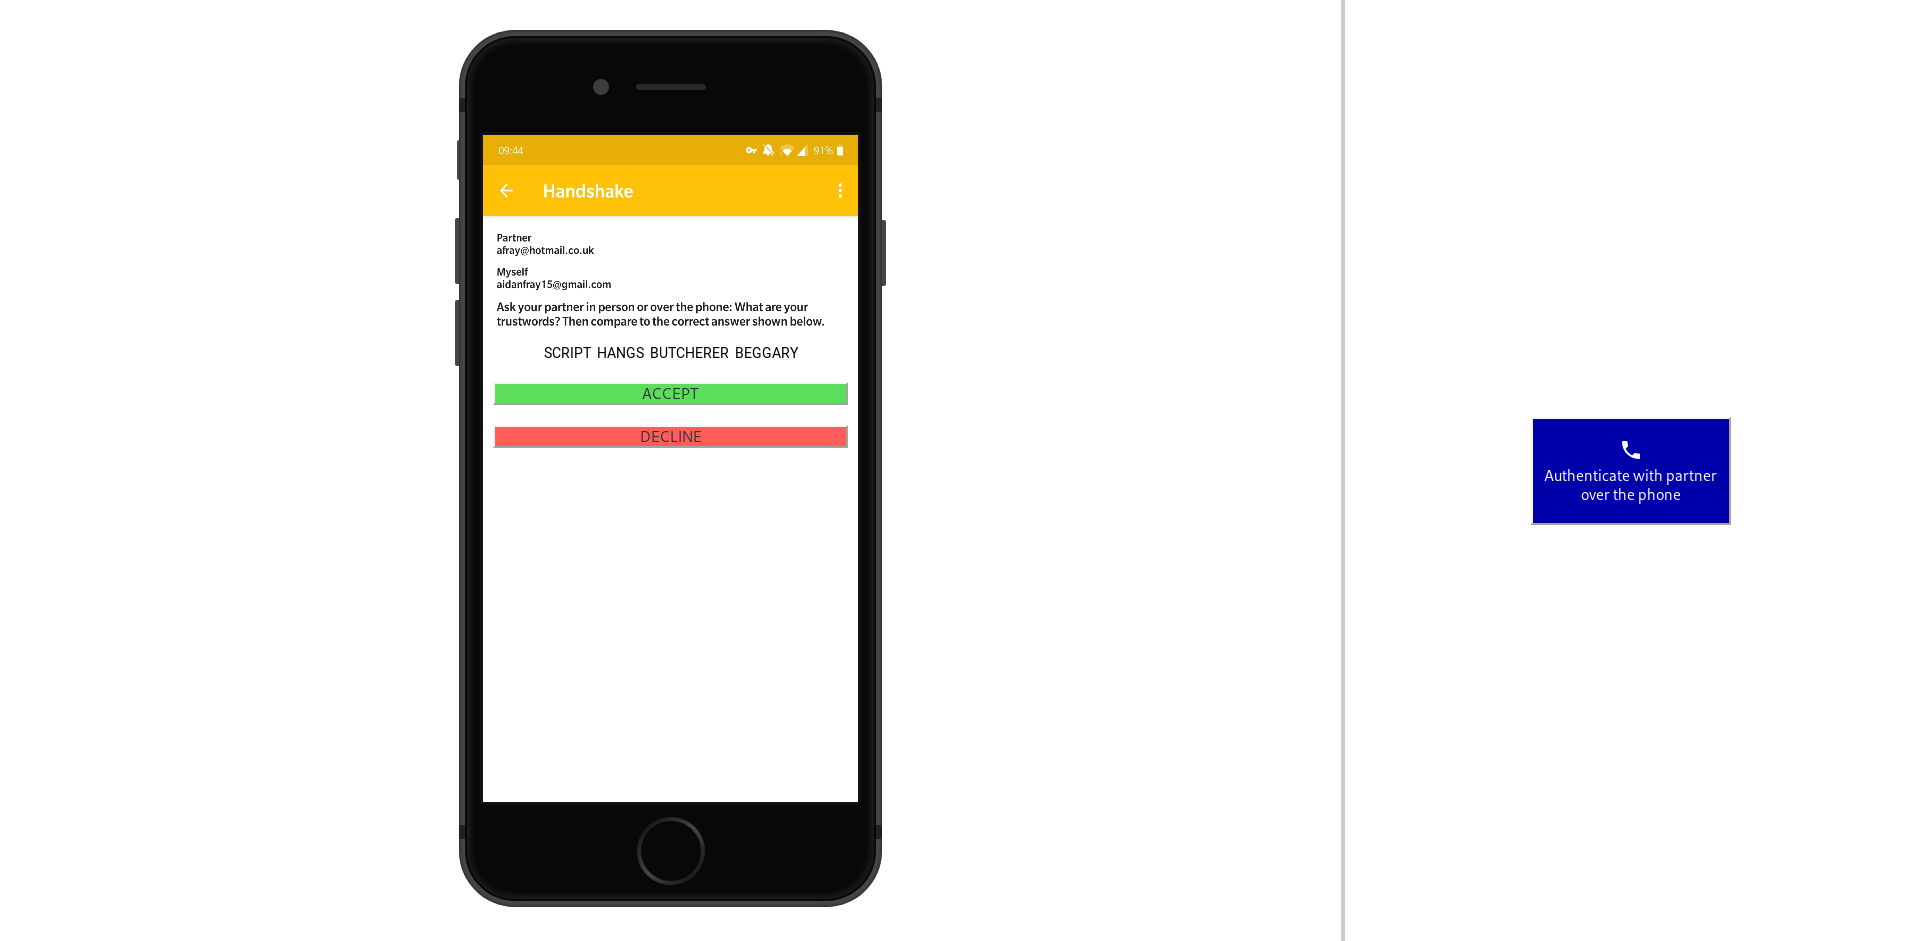
\includegraphics[scale=2.5]{experiment/trustword_attack.png}
    \caption{Experiment UI}
    \label{fig:expID}
\end{figure}

  \printbibliography

\end{document}